\documentclass[10pt]{scrartcl}

%Math
\usepackage{amsmath}
\usepackage{amsfonts}
\usepackage{amssymb}
\usepackage{amsthm}
\usepackage{ulem}
\usepackage{stmaryrd} %f\UTF{00FC}r Blitz!

%PageStyle
\usepackage[ngerman]{babel} % deutsche Silbentrennung
\usepackage[utf8]{inputenc} 
\usepackage{fancyhdr, graphicx}
\usepackage[scaled=0.92]{helvet}
\usepackage{enumitem}
\usepackage{parskip}
\usepackage[a4paper,top=2cm]{geometry}
\setlength{\textwidth}{17cm}
\setlength{\oddsidemargin}{-0.5cm}
\usepackage[scaled=0.92]{helvet}
\usepackage{lastpage} % for getting last page number
\renewcommand{\familydefault}{\sfdefault}
\usepackage{wrapfig}


% Shortcommands
\newcommand{\Bold}[1]{\textbf{#1}} %Boldface
\newcommand{\Kursiv}[1]{\textit{#1}} %Italic
\newcommand{\T}[1]{\text{#1}} %Textmode
\newcommand{\Nicht}[1]{\T{\sout{$ #1 $}}} %Streicht Shit durch

%Arrows
\newcommand{\lra}{\leftrightarrow} 
\newcommand{\ra}{\rightarrow}
\newcommand{\la}{\leftarrow}
\newcommand{\lral}{\longleftrightarrow}
\newcommand{\ral}{\longrightarrow}
\newcommand{\lal}{\longleftarrow}
\newcommand{\Lra}{\Leftrightarrow}
\newcommand{\Ra}{\Rightarrow}
\newcommand{\La}{\Leftarrow}
\newcommand{\Lral}{\Longleftrightarrow}
\newcommand{\Ral}{\Longrightarrow}
\newcommand{\Lal}{\Longleftarrow}

% Code listenings
\usepackage{color}
\usepackage{xcolor}
\usepackage{listings}
\usepackage{caption}
\DeclareCaptionFont{white}{\color{white}}
\DeclareCaptionFormat{listing}{\colorbox{gray}{\parbox{\textwidth}{#1#2#3}}}
\captionsetup[lstlisting]{format=listing,labelfont=white,textfont=white}
\lstdefinestyle{JavaStyle}{
 language=Java,
 basicstyle=\footnotesize\ttfamily, % Standardschrift
 numbers=left,               % Ort der Zeilennummern
 numberstyle=\tiny,          % Stil der Zeilennummern
 stepnumber=5,              % Abstand zwischen den Zeilennummern
 numbersep=5pt,              % Abstand der Nummern zum Text
 tabsize=2,                  % Groesse von Tabs
 extendedchars=true,         %
 breaklines=true,            % Zeilen werden Umgebrochen
 frame=b,         
 %commentstyle=\itshape\color{LightLime}, Was isch das? O_o
 %keywordstyle=\bfseries\color{DarkPurple}, und das O_o
 basicstyle=\footnotesize\ttfamily,
 stringstyle=\color[RGB]{42,0,255}\ttfamily, % Farbe der String
 keywordstyle=\color[RGB]{127,0,85}\ttfamily, % Farbe der Keywords
 commentstyle=\color[RGB]{63,127,95}\ttfamily, % Farbe des Kommentars
 showspaces=false,           % Leerzeichen anzeigen ?
 showtabs=false,             % Tabs anzeigen ?
 xleftmargin=17pt,
 framexleftmargin=17pt,
 framexrightmargin=5pt,
 framexbottommargin=4pt,
 showstringspaces=false      % Leerzeichen in Strings anzeigen ?        
}

 
\fancypagestyle{firststyle}{ %Style of the first page
\fancyhf{}
\fancyheadoffset[L]{0.6cm}
\lhead{

\includegraphics[scale=0.8]{./img/fhnw_logo_en.png}}
\renewcommand{\headrulewidth}{0pt}
\lfoot{school of business,\linebreak www.fhnw.ch }
}

\fancypagestyle{documentstyle}{ %Style of the rest of the document
\fancyhf{}
\fancyheadoffset[L]{0.6cm}
\lhead{

\includegraphics[scale=0.8]{./img/fhnw_logo_en.png}}
\renewcommand{\headrulewidth}{0pt}
\lfoot{\thepage\ / \pageref{LastPage} }
}

\pagestyle{firststyle} %different look of first page
 
\title{ %Titel
Volkswirtschaftslehre
\vspace{0.2cm}
\Large (Zusammenfassung)}

 \begin{document}
 \maketitle
 \thispagestyle{firststyle}
 \pagestyle{firststyle}
 \begin{abstract}
 \begin{center}
  Zusammenfassung des Modul VWL (HS14) von Fabian Stebler. \\
"THE BEER-WARE LICENSE" (Revision 42):\\
fabian.stebler@students.fhnw.ch wrote this file. As long as you retain this notice you
can do whatever you want with this stuff. If we meet some day, and you think
this stuff is worth it, you can buy me a beer in return.
 \end{center}
 \vspace{0.5cm}
\hrulefill
\end{abstract}

 \pagestyle{documentstyle}
 \tableofcontents
 \pagebreak
\section{Grundlagen}
\subsection{Begriffe}
\subsubsection{Volkswirtschaftslehre}
Die Volkswirtschaftslehre oder Ökonomie ist die Wissenschaft vom Einsatz knapper Ressourcen zur Produktion wertvoller Wirtschaftsgüter durch die Gesellschaft und von der Verteilung dieser Güter in der Gesellschaft.
\subsubsection{Effizienz \& Produktionseffizienz}
{\bf Effizienz} bedeutet, die Ressourcen einer Wirtschaft möglichst effektiv einzusetzen, um die Wünsche und Bedürfnisse der Menschen bestmöglich zu befriedigen. \\ \\
Wir sprechen von {\bf Produktionseffizienz}, wenn eine Wirtschaft nicht mehr von einem Gut erzeugen kann, ohne zugleich bei einem anderen Abstriche machen zu müssen, wenn sie sich also auf Ihrer PMK (siehe 1.3.3)befindet. {\bf Produktionsineffizienz} bezeichnet den Zustand einer Wirtschaft, wenn sich diese aus unterschiedlichen Gründen nicht auf der PMK befindet.
\\ \\
{\it Erläuterungen: Das Wesen des Wirtschaftens besteht in der Anerkennung der Knappheit als Realität und in einer gesellschaftlichen Organisation, die einen möglichst effizienten Ressourceneinsatz zulässt.}
\subsubsection{Gut \& Wirtschaftsgut}
Als {\bf Gut } im Allgemeinen bezeichnet man in der Wirtschaftswissenschaft alle Mittel, die der Bedürfnisbefriedigung dienen.

Im engeren Sinn versteht man {\bf Güter} als {\bf Wirtschaftsgüter}; diese werden über ihre Knappheit definiert ("knappe Güter"):
\begin{itemize}
\item es handelt sich um ein Gut, das nicht zu jeder Zeit und an jedem gewünschten Ort in der gewünschten Qualität und Menge zur Verfügung steht.
\item Tausch- und Marktfähigkeit.
\end{itemize}

\subsubsection{Mikroökonomie \& Makroökonomie}
{\bf Mikroökonomie} bezeichenet den Teil der Volkswirtschaft, der sich mit dem Verhalten einzelner Wirtschaftseinheiten wie Märkte, Unternehmen oder Haushalten auseinandersetzt.
Das zweite wichtige Teilgebiet der Volkswirtschaftslehre ist die {\bf Makroökonomie}. Im Gegensatz zur Mikroökonomie arbeitet die Makroökonomie mit aggregierten Größen, also zum Beispiel mit dem Gesamteinkommen aller Haushalte. Heute beschäftigt sich die Makroökonomie mit einer breiten Palette an Themen, etwa mit den Faktoren, die die Investitionen und den Konsum einer Gesellschaft bestimmen, oder mit der Frage, welche Kontrolle die Zentralbanken über Geldmenge und Zinssätze ausüben, was zu internationalen Finanzkrisen führt und warum einige Staaten kräftig wachsen, andere aber stagnieren

\subsubsection{Ökonometrie}
Darüber hinaus haben Ökonomen eine
spezielle Technik, die Ökonometrie, entwickelt, die statistische Methoden auf wirtschaftliche Problemstellungen anwendet. Mithilfe der Ökonometrie können die Wissenschaftler aus riesigen Datenbergen einfache Beziehungen ableiten.
Aber Achtung, wie immer wenn was einfach aussieht:
\begin{itemize}
\item  Der „Post-hoc-Irrtum“. Hier wird zu Unrecht eine Kausalität angenommen, wo
keine besteht.\\
{\it Dieser Irrtum tritt auf, wenn wir aufgrund der zeitlichen Aufeinanderfolge zweier Ereignisse annehmen, das zweite sei durch das erste verursacht worden.} 
\item  Der Irrtum, nicht „alles andere konstant“ zubelassen.\\
{\it Ein weiterer verbreiteter Irrtum ist es, bei der Betrachtung eines Faktors nicht alle anderen Faktoren unverändert zu lassen. }
\item  Der Trugschluss der Verallgemeinerung.\\
{\it Manchmal schließen wir von einem Teil voreilig auf das Ganze. }
\end{itemize}

\subsubsection{Positive vs. Normative Ökonomik}
Die positive Ökonomik beschreibt die Fakten einer Wirtschaft, während sich die normative Ökonomik mit Werturteilen befasst.\\
\begin{itemize}
\item {\bf positive Ökonomik}\\
Fragen die sich mit gründlicher Analyse und mithilfe empirischer Daten lösen lassen.
\item {\bf normative Ökonomik}\\
In der normativen Ökonomik geht es um ethisches Verhalten und Normen der Fairness.

\end{itemize}
{\it 
BSP:\\
positiv: Warum verdienen Ärzte mehr als Maurer?\\
normativ: Sollten Bedürftige vom Staat, der sie unterstützt, zum Arbeiten angehalten werden?\\}
\subsection{Die 3 Grundfragen der Wirtschaft}
\begin{itemize}
\item {\bf Was} wird produziert und in welchen Mengen? 
\item {\bf Wie} wird produziert?
\item Für {\bf wen} wird produziert?
\end{itemize}
\subsubsection{ Marktwirtschaft, Planwirtschaft, Mischwirtschaft}
Die drei Grundfragen werden von den Volkswirtschaften verschieden
beantwortet.\\
Man unterscheidet zwischen zwei grundlegend verschiedenen Organisationsformen (Wirtschaftssysteme) einer Wirtschaft:
\begin{itemize}
\item In der Planwirtschaft werden die Grundfragen wie, was und für wen produzieren vom Staat entschieden.
\item In der Marktwirtschaft fallen die Entscheidungen auf den Märkten, wo sich Einzelpersonen (Haushalte) oder Unternehmen freiwillig über den Einsatz von Ressourcen (Input) und das Produktionsergebnis (Output) einigen. Preise, Märkte, Gewinne und Verluste, Anreize und Belohnungen über das Was, Wie und für Wen.
\item Die reinen Formen existieren nicht. Alle Volkswirtschaften verfügen über ein Mischsystem mit Elementen aus Markt- und Planwirtschaft.
\end{itemize}
\subsection{Die Technologischen Möglichkeiten einer Gesellschaft}
\subsubsection{Input, Output}
\begin{itemize}
\item {\bf Inputs} sind Waren oder Dienstleistungen, die ihrerseits der Erzeugung von Gütern und Dienstleistungen dienen. Eine Wirtschaft setzt die ihr zur Verfügung stehenden Technologien ein, um mit Hilfe der Inputs Outputs zu erzeugen.
\item {\bf Outputs } sind die verschiedenen nützlichen Güter und Dienstleistungen, die aus der Produktion hervorgehen und die entweder konsumiert oder im weiteren Produktionsprozess eingesetzt werden.
\end{itemize} 
\subsubsection{Produktionsfaktoren}
\begin{itemize}
\item {\bf natürliche Ressourcen} (Grund und Boden)\\
Zum Produktionsfaktor Boden gehören die Felder, auf denen wir unsere Landwirtschaft betreiben, oder die Grundstücke für unsere Häuser, Fabriken und Straßen; in
diese Kategorie fallen aber auch Energieressourcen für unsere Autos, Heizungen oder Haushalte sowie Bodenschätze wie Kupfer, Erz oder Sand. In einer immer dichter besiedelten Welt müssen wir die Palette natürlicher Ressourcen um Umweltressourcen wie saubere Luft und Trinkwasser erweitern.
\item {\bf Arbeit} \\
Arbeit  als Produktionsfaktor bedeutet die Zeit, die Menschen für die Produktion aufwenden.
\item {\bf Kapital} \\
Kapital beinhaltet jene dauerhaften Güter einer Wirtschaft, die produziert werden, damit andere Güter erzeugt werden können. Zu den Kapital- oder Investitionsgütern gehören Maschinen, Straßen, Computer, Hämmer, LKWs, Stahlwerke, Autos, Waschmaschinen und Gebäude. Wie wir später noch sehen werden, ist es für die wirtschaftliche Entwicklung unabdingbar, einen Grundstock an spezialisierten Investitionsgütern anzusammeln.
\end{itemize}

\subsubsection{Transformations- oder Produktionsmöglichkeitenkurve (PMK) }
\begin{wrapfigure}{l}{0.4\textwidth}
  \begin{center}
    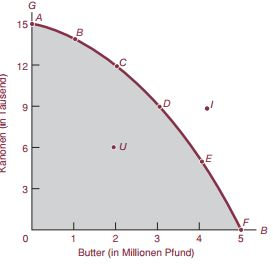
\includegraphics[width=0.38\textwidth]{img/pmk.jpg}
  \end{center}
  \caption{\it Produktionsmöglichkeitenkurve (PMK)}
\end{wrapfigure}
Die Transformations- oder Produktionsmöglichkeitenkurve (PMK) zeigt die maximalen Produktionsmengen, die eine Wirtschaft angesichts ihres technologischen Know-how's und der verfügbaren Menge an Produktionsfaktoren erzielen kann. Die PMK stellt die Gesamtheit der Güter und Dienstleistungen dar, die eine Gesellschaft produzieren kann.\\
{\it Produktionsmöglichkeiten- oder Transformationskurven veranschaulichen eine Vielzahl grundlegender öko-nomischer Prozesse: wie das Wirtschaftswachstum die PMK nach außen verschiebt, wie ein Staat im Zuge seiner Entwicklung vergleichsweise immer weniger Nahrungsmittel und andere lebensnotwendige Güter erzeugt, wie ein Land zwischen privaten und öffentlichen Gütern zu wählen hat und wie sich Gesellschaften zwischen Konsumgütern und Kapitalgütern, die den künftigen Konsum erhöhen, entscheiden müssen.\\
Gesellschaften befinden sich bisweilen innerhalb ihrer PMK. Bei hoher Arbeitslosigkeit oder wenn Unruhen oder ineffiziente staatliche Maßnahmen die Wirtschaftsaktivitäten hemmen, wird die Wirtschaft ineffizient und fällt daher hinter ihre PMK zurück.}\\
\subsubsection{Opporunitätskosten}
In einer Welt der Knappheit bedeutet die Wahl einer Möglichkeit immer den Verzicht auf eine andere. Die {\bf Opportunitätskosten } einer Entscheidung entsprechen dem Wert des nicht gewählten Gutes oder der nicht gewählten Dienstleistung.\\
{\it Tauschware Zeit \\
 Eine der wichtigsten Entscheidungen, die Menschen treffen müssen, betrifft den Einsatz ihrer Zeit. Für sämtliche Aktivitäten, denen Leute nachgehen, steht ihnen immer nur ein beschränktes Angebot an Zeit zur Verfügung. }
 \pagebreak
 
 
\section{Markt und Staat in der modernen Wirtschaft}
\subsection{Markt}
Ein {\bf Markt} ist ein Mechanismus, mit dessen Hilfe Käufer und Verkäufer miteinander in Beziehung treten, um Preis und Menge einer Ware oder Dienstleistung zu ermitteln.
\subsubsection{Preis(e)}
{\bf Preise} koordinieren die Entscheidungen von Produzenten und Konsumenten auf einem Markt. Höhere Preise dämpfen zumeist die Nachfrage bei den Konsumenten und kurbeln gleichzeitig die Produktion an. Geringere Preise hingegen fördern die Kauflust der Leute und wirken sich hemmend auf die Produktion aus. Preise sind also das ausgleichende Element im Marktmechanismus.
\subsubsection{Marktgleichgewicht}
Das Marktgleichgewicht stellt den Ausgleich zwischen all den verschiedenen Käufern und Verkäufern her. Der Markt ermittelt den Gleichgewichtspreis, der sowohl die Wünsche der Käufer als auch jene der Verkäufer berücksichtigt.\\
{\bf Wie lösen Märkte die drei Grundfragen der Volkswirtschaft?}
\begin{itemize}
\item {\bf Was} produziert wird (also welche Güter und Dienstleistungen), entscheiden letztlich die Konsumenten, deren Geldausgaben als eine Art „Stimmzettel“ fungieren.
\item {\bf Wie} produziert wird, entscheidet sich durch den Wettbewerb zwischen verschiedenen Produzenten. Die beste Möglichkeit für die Produzenten, die Preiskonkurrenz zu bestehen und die eigenen Gewinne zu maximieren, besteht in einer Minimierung ihrer Kosten durch den Einsatz möglichst effizienter Produktionsmethoden.
\item {\bf Für wen } produziert wird – also wer konsumiert und wie viel –, hängt weitgehend von Angebot und Nachfrage auf den Faktormärkten ab. Faktormärkte (die Märkte für Produktionsfaktoren) bestimmen die Höhe der Löhne und Pachten, Zinssätze und Gewinne. Die zugehörigen Preise heißen daher {\it Faktorpreise}
\end{itemize}

    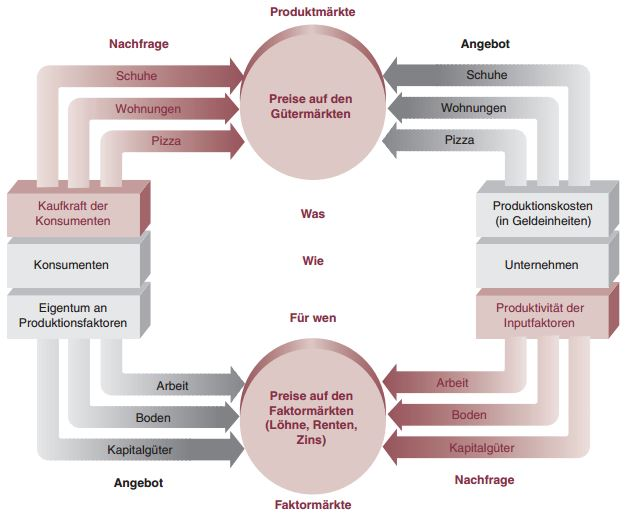
\includegraphics[width=0.5\textwidth]{img/markt.jpg}

Wir sehen hier den Kreislauf einer Marktwirtschaft. Die Kaufentscheidungen der Konsumenten (also von Haushalten, öffentlicher Hand und Ausländern) treten in eine Wechselwirkung zum Angebot auf den Gütermärkten (oben) und bestimmen dadurch mit, was produziert wird. Die Unternehmensnachfrage nach Produktionsfaktoren oder Inputs trifft auf den Faktormärkten (unten) auf das Arbeitsangebot und sonstige Inputs, wodurch Löhne, Renten und Zinsen bestimmt werden; auf diese Weise beeinflussen die Einkommen, für wen produziert wird. Der Wettbewerb zwischen den Unternehmen in Bezug auf den möglichst billigen Kauf von Faktorinputs und Verkauf von Gütern entscheidet darüber, wie Güter produziert werden. \\
\subsubsection{Die unsichtbare Hand}
Adam Smith hat eine ganz bemerkenswerte Eigenschaft der wettbewerbsorientierten Marktwirtschaft entdeckt. Unter den Bedingungen des vollständigen Wettbewerbs, und sofern es zu keinem Marktversagen kommt, gelingt es den Märkten, das Maximum an nützlichen Gütern und Dienstleistungen aus den vorhandenen Ressourcen herauszuholen. Wo jedoch Monopole, Umweltverschmutzung oder ähnliche Formen von Marktversagen auftreten, kann dies die bemerkenswerte Effizienz der unsichtbaren Hand untergraben. 

\subsection{Handel, Geld und Kapital}
Reife, entwickelte kapitalistische Volkswirtschaften zeichnen sich durch drei wesentliche Merkmale aus: Handel und Spezialisierung, Geld und Sachkapital.
\begin{itemize}
\item Eine entwickelte Volkswirtschaft verfügt über ein komplexes Handelsnetz zwischen den agierenden Personen und Ländern, das erst mit massiver Spezialisierung und ausgeklügelter Arbeitsteilung möglich wird.
\item Die heutigen, modernen Volkswirtschaften arbeiten in hohem Maße mit Geld oder
anderen Zahlungsmitteln.
\item Die Technologien unserer modernen Industrie beruhen auf dem Einsatz riesiger Mengen an Sachkapital: Präzisionsmaschinen, Großraumfabriken, Lagerbestände
\end{itemize}
\subsubsection{Handel, Spezialisierung und Arbeitsteilung}
Entwickelte Volkswirtschaften bemühen sich um Spezialisierung und Arbeitsteilung, wodurch sie die Produktivität ihrer Ressourcen erhöhen. Einzelpersonen und Länder tauschen freiwillig jene Produkte, auf deren Herstellung sie sich spezialisiert haben, gegen die Produkte anderer und vergrößern auf diese Weise sowohl die Bandbreite als auch die Menge der konsumierten Güter enorm, wodurch in der Folge der Lebensstandard aller steigt.
\subsubsection{Geld}
Geld ist ein Tauschmittel. Der richtige Umgang mit der Geldmenge gehört zu den wichtigsten Aufgaben der Wirtschaftspolitik aller Staaten.
\subsubsection{Kapital}
In der Wirtschaft geht es unter anderem darum, auf sofortigen Konsum zu verzichten und stattdessen das vorhandene Kapital zu vermehren. Jedes Mal, wenn wir etwas investieren – eine neue Fabrik oder Straße bauen, die Ausbildung verlängern oder qualitativ verbessern oder unsere Bestände an nutzbarer Technologie und Know-how erhöhen –, fördern wir die künftige Produktivität unserer Wirtschaft und damit auch den künftigen Konsum.\\
\\
\subsubsection{Kapital und Privateigentum}
In einer Marktwirtschaft befindet sich Kapital zumeist in Privateigentum, und der Einzelne bezieht ein Einkommen aus seinem Kapital. Für jeden Flecken Land gibt es eine Übertragungsurkunde oder einen Eigentumstitel; beinahe jede Maschine und jedes Gebäude gehört einem einzelnen Menschen oder einem Unternehmen. Eigentumsrechte verleihen den Eigentümern die Möglichkeit, ihre Kapitalgüter nach ihrem Ermessen zu verwenden, auszutauschen, anzustreichen, auszugraben, anzubohren oder auszubeuten. Diese Kapitalgüter haben auch einen Marktwert, und man kann sie zu jedem beliebigen erzielbaren Preis auf dem Markt kaufen und verkaufen. Diese Möglichkeit des Einzelnen, Kapital zu besitzen und daraus Nutzen zu ziehen, gibt dem Kapitalismus seinen Namen.

\subsubsection{Moderne Volkswirtschaft}
Eine moderne Volkswirtschaft muss ganz spezielle Eigenschaften aufweisen, um möglichst
produktiv zu sein. Arbeitsteilung und hoch spezialisiertes Kapital erlauben es dem Einzelnen, sich selbst auf einem bestimmten Gebiet zu spezialisieren. Doch all die spezialisierten Individuen, Unternehmen und Länder können nur überleben, weil der mit Geld geschmierte Handel es verschiedenen Personen und Ländern erlaubt, ihre Produkte problemlos zu verkaufen und ebenso problemlos das Nötige einzukaufen. Die Spezialisierung hat eine enorme Effizienz zur Folge; die gesteigerte Produktion ermöglicht den Handel; das Geld macht diesen Handel schnell und effizient; und ein ausgeklügeltes Finanzsystem dient dazu, die Ersparnisse einiger in das Kapital anderer zu verwandeln.

\subsection{Die Rolle des Staates in der Wirtschaft}
Staaten haben in einer Marktwirtschaft drei wesentliche wirtschaftliche Funktionen: Die Erhöhung der Effizienz, die Förderung der sozialen Gerechtigkeit und die Sicherung von volkswirtschaftlicher Stabilität und Wachstum.
\subsubsection{Effizienz}
Eine schwerwiegende Abweichung vom effizienten Markt stellt der {\bf unvollständige Wettbewerb oder das Monopol} dar. Während im vollständigen Wettbewerb weder einzelne Unternehmen noch einzelne Konsumenten Einfluss auf die Preisbildung nehmen können, sprechen wir von unvollständigem Wettbewerb, wenn ein einzelner Käufer oder Verkäufer in der Lage ist, Einfluss auf den Preis einer Ware oder Dienstleistung zu nehmen.\\
{\bf Externe Effekte (oder Spillover-Effekte)} treten auf, wenn die wirtschaftliche Aktivität von Unternehmen oder Individuen bei marktfernen Akteuren zu Kosten oder einem Nutzen führt. (z.B. Flughafenlärm)\\
{\bf öffentliche Güter} Ein klassisches Beispiel dafür ist die Armee eines Landes. Wenn
ein Land in den Krieg zieht – um Terroristen zu bekämpfen, Massenvernichtungswaffen zusuchen, um Land oder Öl zu stehlen oder patriotische Gefühle in der Bevölkerung zu schüren –, müssen alle die Zeche zahlen, ob sie wollen oder nicht. 
\subsubsection{Soziale Gerechtigkeit}
Die Märkte produzieren nicht notwendigerweise eine sozial gerechte Einkommensverteilung. Eine Marktwirtschaft kann sogar völlig inakzeptable Ungleichheiten bei Einkommen und Konsum hervorbringen.
\subsubsection{Wirtschaftswachstum und Stabilität}
\begin{wrapfigure}{l}{0.5\textwidth}
  \vspace{-20pt}
  \begin{center}
    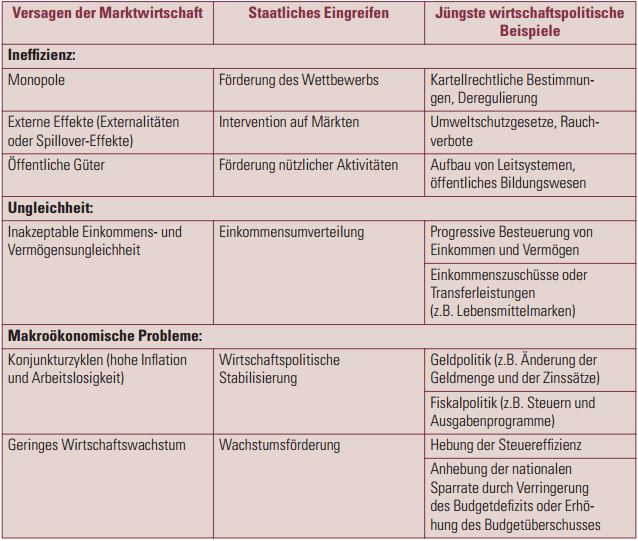
\includegraphics[width=0.48\textwidth]{img/staat.jpg}
  \end{center}
   \vspace{-10pt} 
\end{wrapfigure}
Durch den umsichtigen Einsatz {\bf fiskal- und geldpolitischer Maßnahmen} können die Staaten Produktivität, Beschäftigung und Inflation wirksam beeinflussen. Unter der Fiskalpolitik eines Staates versteht man dessen Möglichkeit, Steuern zu erheben und Ausgaben zu tätigen. Als Geldpolitik bezeichnet man hingegen die Festlegung der Geldmenge und der Zinssätze. \\
Makroökonomische Strategien zur Stabilisierung und Förderung des Wirtschaftswachstums beinhalten fiskal- oder haushaltspolitische Maßnahmen (Steuereinnahmen und Staatsausgaben) ebenso wie geldpolitische Maßnahmen (Einflussnahme auf Zinssätze und Kreditkonditionen). Seit der Entwicklung der Makroökonomie in den 1930er Jahren konnten Staaten immer wieder erfolgreich die schlimmsten Exzesse von Inflation und Arbeitslosigkeit eindämmen.









\pagebreak
\newpage
\section{Angebot und Nachfage}
\subsection{Nachfragefunktion}
Die Beziehung zwischen Preis und gekaufter Menge wird als Nachfragefunktion oder Nachfragekurve bezeichnet.
\subsubsection{Das Gesetz des negativen Nachfrageverlaufs}
Wenn der Preis für eine Ware angehoben wird (und alle anderen Faktoren gleich bleiben), neigen die Käufer dazu, weniger von dieser Ware zu kaufen. Ebenso erhöht sich, wenn der Preis gesenkt wird und alle anderen Einflussfaktoren unverändert bleiben, die nachgefragte Menge.
\subsubsection{Substitutions- / Einkommenseffekt}
\begin{itemize}
\item {\bf Substitutionseffekt }Sobald der Preis einer Ware steigt, werde ich versuchen, diese Ware durch eine andere zu ersetzen.  
\item Der {\bf Einkommenseffekt} kommt ins Spiel, weil ein erhöhter Preis etwas ärmer macht. Der Versuch weniger von einer Ware zu konsumieren beginnt.
\end{itemize}
\subsubsection{Marktnachfrage / -kurve}
Die Marktnachfragekurve lässt sich durch Addition der von allen Konsumenten zu jedem Preis nachgefragten Mengen ermitteln.
\subsubsection{Kräfte hinter der Nachfragekurve}
\begin{itemize}
\item {\bf Durchschnittseinkommen} Mit steigenden Einkommen kaufen die Leute mehr.
\item {\bf Bevölkerungszahl } Eine Zunahme der Bevölkerung treibt die Verkaufszahlen nach oben.
\item {\bf Preise verwandter Güter} Niedrigere Preise erhöhen die Nachfrage auf Gut.
\item {\bf Präferenzen } Trend, Statussymbol.
\item {\bf Spezielle Einflüsse }  Verkehrsaufkommen in Städten, Umwelt, usw.
\end{itemize}

Wenn sich andere Einflussfaktoren auf das Kaufvolumen als der Preis einer Ware ändern, sprechen wir von einer Nachfrageverschiebung. Die Nachfrage steigt (oder sinkt), wenn die zu jedem Preis nachgefragte Menge steigt (oder sinkt). 

{\bf Bewegung entlang einer Kurve oder Verschiebung der Kurve selbst? }\\
Verwechseln Sie bitte nie Bewegungen entlang von Kurven mit Kurvenverschiebungen. Unterscheiden Sie unbedingt zwischen einer Veränderung der Nachfrage (und somit einer Verschiebung der Nachfragekurve) und einer Veränderung der nachgefragten Menge (also der Bewegung hin zu einem  anderen Punkt auf derselben Nachfragekurve infolge einer Preisänderung).  Eine Änderung der Nachfrage ergibt sich, sobald sich einer der Faktoren, die der  Nachfragekurve zugrunde liegen, verändert.
\subsection{Angebotsfunktion}
Die Angebotsfunktion (oder die Angebotskurve) eines Gutes stellt die Beziehung zwischen seinem Marktpreis und jener Menge dieses Gutes dar, die die Produzenten zu produzieren und zu verkaufen gewillt sind,  wenn alle anderen Faktoren konstant bleiben.
\subsubsection{Kräfte hinter der Angebotskurve}
\begin{itemize}
\item {\bf Technologie } Neue Maschienen senken Produktionskosten
\item {\bf Faktorpreise } Niedrigere Löhne der Arbeiter senken die Produktionskosten und erhöhen das Angebot.
\item {\bf Preise verwandter Güter } Sinkende Preise von ähnlichen Gütern sinken
\item {\bf Wirtschaftspolitische Maßnahmen } Die Beseitigung von Importquoten und Zöllen auf importierte Güter.
\item {\bf Spezielle Einflüsse } Einkäufe und Auktionen im Internet ermöglichen den Konsumenten einen einfachen Preisvergleich zwischen den Anbietern und vertreiben teure Anbieter vom Markt.
\end{itemize}
Wenn die Angebotsmenge von anderen Faktoren als dem Preis einer Ware beeinflusst wird, sprechen wir von einer Angebotsverschiebung. Das Angebot steigt (oder sinkt), wenn die zu jedem Marktpreis angebotene Menge steigt (oder sinkt).
\subsection{Marktgleichgewicht und Gleichgewichtspreis}
\begin{wrapfigure}{l}{0.5\textwidth}
  \begin{center}
    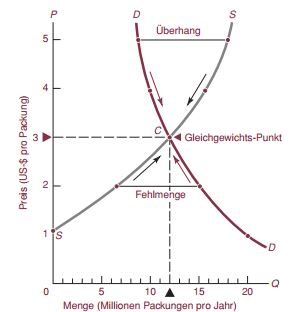
\includegraphics[width=0.4\textwidth]{img/angebot_nachfrage_1.jpg}
  \end{center}
\end{wrapfigure}
Ein {\bf Marktgleichgewicht} stellt sich bei dem Preis ein, bei dem die nachgefragte Menge der angebotenen Menge entspricht. Bei diesem Gleichgewicht gibt es keine Preistendenzen nach oben oder unten. Der Gleichgewichtspreis wird auch Markträumungspreis genannt. Damit soll ausgedrückt werden, dass bei diesem Preis alle Angebots- und Nachfragevorstellungen befriedigt werden, dass die Auftragsbestände in den Büchern ausgeglichen sind und dass Konsumenten wie auch Produzenten rundum zufrieden sind.
\\
\\
{\bf Gleichgewichtspreis} und {\bf Gleichgewichtsmenge }stellen sich dort ein, wo die freiwillig angebotene der freiwillig nachgefragten Menge entspricht. Auf einem vollkommenen Markt tritt dieses Gleichgewicht im Punkt der Überschneidung von Angebots- und Nachfragekurve ein. Zum Gleichgewichtspreis gibt es weder einen Überhang noch eine Fehlmenge.
\\
\\
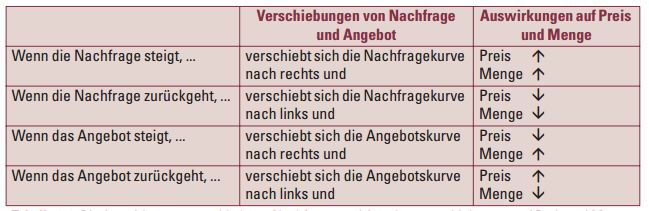
\includegraphics[width=0.75\textwidth]{img/angebot_nachfrage_bewegungen.jpg}
\pagebreak
\section{Anwendungsgebiete Angebots- und Nachfrageanalyse}
\subsection{Preiselastizität von Angebot und Nachfrage}
Damit aus der Theorie von Angebot und Nachfrage ein wirklich brauchbares Werkzeug entsteht, müssen wir wissen, wie stark Angebot und Nachfrage auf Preisänderungen reagieren. Bestimmte Kaufentscheidungen, wie zum Beispiel Urlaubsreisen, sind von Preisänderungen sehr leicht beeinflussbar.Die Elastizität ist tendenziell höher, wenn es sich um Luxusgüter handelt, wenn Ersatzgüter verfügbar sind und wenn die Konsumenten länger Zeit haben, um ihr Verhalten anzupassen. Andere Güter, wie Lebensmittel oder elektrischer Strom, sind Notwendigkeiten des täglichen Lebens, was bedeutet, dass die Kaufbereitschaft der Konsumenten in diesem Sektor kaum auf Preisänderungen reagiert.
\\
Die {\bf Preiselastizität der Nachfrage, Preiselastizität} misst, inwieweit sich die nachgefragte Menge eines Gutes infolge von Preisänderungen verändert.
\subsection{Preiselastizität der Nachfrage}
\begin{equation}
\text{{\bf Preiselastizität der Nachfrage}} = \frac{\text{prozentuale Änderung der nachgefragten Menge}}{\text{prozentuale Preisänderung}} \nonumber
\end{equation}\\
\begin{equation}
E_{D} =  \frac{ \Delta Q }{\frac{(Q_{1} + Q_{2})}{2}} \div \frac{ \Delta P }{\frac{(P_{1} + P_{2})}{2}} \nonumber
\end{equation}
{\it wobei P1 und Q1 den ursprünglichen Preis und die ursprüngliche Menge und P2 und Q2 den neuen Preis und die neue Menge bezeichnen.}\\
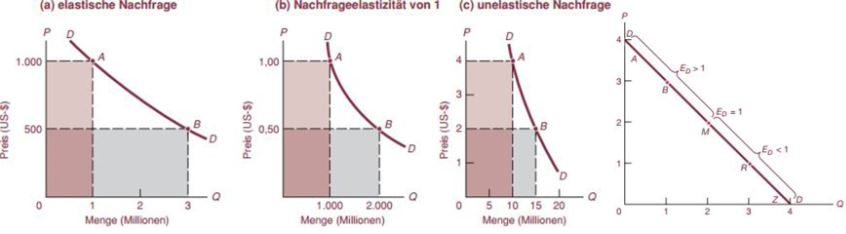
\includegraphics[width=0.95\textwidth]{img/elastizitaten.jpg}
\begin{itemize}
\item {\bf preiselastischen Nachfrage:} Wenn eine einprozentige Preisänderung eine mehr als einprozentige Änderung der nachgefragten Menge nach sich zieht, ist die Preiselastizität der
Nachfrage dieses Gutes sehr hoch.
\item {\bf preisunelastischen Nachfrage:} Wenn eine einprozentige Preisänderung eine weniger als einprozentige Änderung der nachgefragten Menge nach sich zieht.
\item Ein wichtiger Sonderfall liegt vor, wenn die Elastizität der Nachfrage den Wert 1 annimmt, wenn also die prozentuale Mengenänderung genau so groß ist wie die prozentuale Preisänderung. Dies impliziert, dass die Gesamtausgaben für das betreffende Wirtschaftsgut trotz Preisänderung gleich bleiben.
\item Alle Punkte auf der gerade verlaufenden Nachfragekurve haben dieselbe Steigung. Hingegen ist die Nachfrage oberhalb von Punkt M elastisch, darunter jedoch unelastisch. Im Mittelpunkt beträgt die Nachfrageelastizität 1.
\end{itemize}
\pagebreak
\subsubsection{Kurzmethode zur Berechnung}
\begin{wrapfigure}{L}{0.18\textwidth}
\vspace{-20pt}
  \begin{center}
    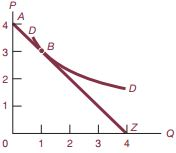
\includegraphics[width=0.16\textwidth]{img/kurzmethode_elas.jpg}
  \end{center}
  \vspace{-20pt}
\end{wrapfigure}
Die Nachfrageelastizität ergibt sich durch das Verhältnis der Länge des geraden Linienabschnitts unterhalb des Punktes zur Länge des Linienabschnitts oberhalb des Punktes. Das bedeutet, dass die Elastizität bei Punkt B mit 3 berechnet werden kann. Für nicht lineare Nachfragekurven zeichnen Sie einfach die Tangente und berechnen Sie ihre Elastizität.\\

\subsection{Elastizität und Ertrag}
Der Gesamtertrag ist definiert als Preis mal Menge (oder P x Q). Kaufen die Konsumenten 5 Einheiten eines Gutes zu je CHF 3, beträgt der Gesamtertrag CHF 15. Wenn Sie die Preiselastizität der Nachfrage kennen, wissen Sie jetzt auch, wie sich der Gesamtertrag nach einer Preisänderung entwickeln wird:
\begin{itemize}
\item Bei preisunelastischer Nachfrage verringert eine Preissenkung den Gesamtertrag.
\item Bei preiselastischer Nachfrage erhöht eine Preissenkung den Gesamtertrag.
\item Im Grenzfall der Nachfrageelastizität von 1 bewirkt eine Preissenkung keinerlei Veränderung des Gesamtertrages
\end{itemize}
\subsection{Preiselastizität der Angebots}
Die Preiselastizität des Angebots misst die prozentuale Änderung des von den Produzenten gelieferten Outputs, wenn sich der Marktpreis um einen bestimmten Prozentsatz ändert.
\begin{equation}
\text{{\bf Preiselastizität des Angebots}} = \frac{\text{prozentuale Änderung der angebotenen Menge}}{\text{prozentuale Preisänderung}} \nonumber
\end{equation}\\
\subsection{Anwendung auf wichtige ökonomische Fragen}
Ein besonders anschauliches Gebiet zum Studium der Wirkungsweise von Angebot und Nachfrage ist die Landwirtschaft. Verbesserungen in der Agrartechnologie bedeuten, dass das Angebot stark steigt, während die Nachfrage nach Lebensmitteln weniger zunimmt, als den Einkommenssteigerungen der Konsumenten entsprechen würde. Daher fallen die Preise für Nahrungsmittel auf dem freien Markt tendenziell. Kein Wunder also, dass viele Staaten eine ganze Reihe von Programmen eingeführt haben, etwa Flächenstilllegungen, um die Einkommen ihrer Landwirte anzuheben.
\\ \\ 
Eine Produktsteuer (Verbrauchssteuer auf ein Wirtschaftsgut) verschiebt das Gleichgewicht von Angebot und Nachfrage. Die Steuerlast (oder die Wirkung auf die Einkommen) trifft die  Konsumenten in dem Ausmaß stärker als die Produzenten, in dem die Nachfrage im Vergleich zum Angebot unelastisch ist.
\\ \\
{\bf Izidenz: }  Mit Inzidenz meinen wir die letztendliche Auswirkung einer Steuer auf die Realeinkommen der Produzenten oder Konsumenten. 
\\ \\
Staaten greifen von Zeit zu Zeit in die Mechanismen der Wettbewerbsmärkte ein, indem sie Höchst- oder Mindestgrenzen für Preise festsetzen. In einer solchen Situation muss die angebotene Menge nicht mehr  der nachgefragten Menge entsprechen; Preisobergrenzen führen zu einem Nachfrageüberschuss, während Preisuntergrenzen einen Angebotsüberschuss zur Folge haben. Manchmal kann der Eingriff die Einkommen einer bestimmten Gruppe erhöhen,  wie es bei Landwirten oder bei Arbeitskräften in Niedriglohnbranchen der Fall ist. Verzerrungen und Ineffizienz sind oft die Folge.
\section{Nachfrage und Konsumverhalten}
\subsection{Nutzen}
{\bf Nutzen} bedeuted Berdürfnissbefriedigung. Genauer gesagt, beschreibt der Begriff,wie die Konsumenten verschiedene Güter und Dienstleistungen bewerten. Der Begriff des Nutzens ist ein wissenschaftliches Konstrukt, das es den Ökonomen ermöglicht zu verstehen, wie die Konsumenten ihre beschränkten Ressourcen auf die Waren verteilen, die ihre Bedürfnisse befriedigen.\\
Das {\bf Gesetz des abnehmenden Grenznutzens} besagt, dass der Grenznutzen mit zunehmender Menge eines konsumierten Gutes in aller Regel abnimmt.\\ 
\\
Der Begriff „Grenz-“ ist in der „Volkswirtschaftslehre von größter Bedeutung, und er wird immer im Sinne von „zusätzlich“ verwendet. Der Grenznutzen beschreibt den zusätzlichen Nutzen, den Ihnen der Konsum einer zusätzlichen Einheit eines Gutes verschafft. \\
\begin{wrapfigure}{l}{0.5\textwidth}
\vspace{-20pt}
  \begin{center}
    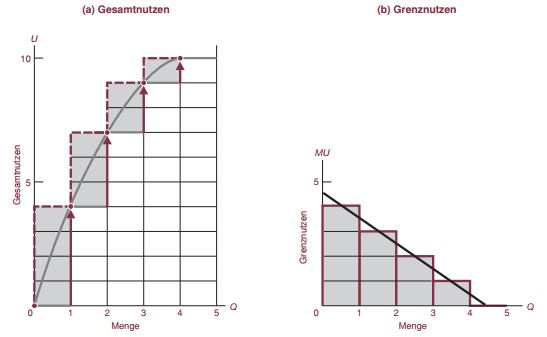
\includegraphics[width=0.48\textwidth]{img/nutzen.jpg}
  \end{center}
  \vspace{-10pt}
\end{wrapfigure}
Der Gesamtnutzen in (a) steigt mit dem Konsum, aber er steigt nicht genauso stark wie der Konsum, was den abnehmenden Grenznutzen signalisiert. Diese Beobachtung hat die Ökonomen früherer Zeiten dazu bewogen, das Gesetz des negativen Nachfrageverlaufs zu formulieren. Die grauen Blöcke zeigen den durch jede neu hinzukommende Einheit bewirkten Zusatznutzen. Die Tatsache, dass der Gesamtnutzen in immer geringerem Maß steigt, wird in (b) durch die abwärts verlaufenden Stufen des Grenznutzens dargestellt. Wenn wir unsere Einheiten immer kleiner machen, werden die Stufen letztlich geglättet, sodass der Gesamtnutzen zu der  durchgehenden schwarzen Kurve in (a) wird. Außerdem lässt sich der durchgehende Grenznutzen, der in (b) durch die schwarze abfallende Kurve dargestellt wird, von der Steigung der durchgehenden Kurve in (a) nicht unterscheiden. \\
\subsection{Prinzip des gleichen Grenznutzens}
Die grundlegende Bedingung für die größtmögliche Bedürfnisbefriedigung oder den größtmöglichen Nutzen ist {\bf das Prinzip des gleichen Grenznutzens}. Laut diesem Prinzip erzielt ein Konsument mit einem gegebenen Einkommen, der mit gegebenen Marktpreisen konfrontiert ist, die maximale Bedürfnisbefriedigung oder den maximalen Nutzen, wenn der Grenznutzen der letzten für jedes Gut ausgegebenen Geldeinheit genau derselbe ist wie der Grenznutzen der letzten für ein anderes Gut ausgegebenen Geldeinheit.\\
\begin{equation}
\text{MU (Grenznutzen) pro Geldeinheit/Einkommen} = \frac{MU_{Gut1}}{P_{1}} = \frac{MU_{Gut2}}{P_{2}} = \frac{MU_{Gut3}}{P_{3}} \nonumber
\end{equation}\\
Der durchschnittliche Grenznutzen pro Geldeinheit aller Güter im Konsumgleichgewicht wird als {\bf Einkommens-Grenznutzen} bezeichnet.\\
Ein höherer Preis für ein Gut reduziert den vom Konsumenten gewünschten Konsum dieses Gutes; dies zeigt, warum die Nachfragekurve negativ verläuft und daher fällt.

\subsection{Alternative: Substitutions- und Einkommenseffekt}
\subsubsection{Substitutionseffekt}
Der {\bf Substitutionseffekt} besagt, dass der Konsument bei steigendem Preis eines Gutes
dazu tendiert, dieses teurere Gut durch andere Güter zu ersetzen, um seine Bedürfnisse auf billigere Weise zu befriedigen.
\subsubsection{Einkommenseffekt}
Der {\bf Einkommenseffekt} bezeichnet die Auswirkung einer Preisänderung auf die nachgefragte Menge eines Gutes, die infolge der Veränderung der realen Einkommen der Konsumenten eintritt. \\
Um ein quantitatives Maß für den Einkommenseffekt zu erhalten, untersuchen wir die
{\bf Einkommenselastizität } eines Gutes. Einkommenselastizität bedeutet die relative, also prozentuale Änderung der nachgefragten Menge dividiert durch die prozentuale Änderung des Einkommens, wobei alle anderen Faktoren, beispielsweise die Preise, konstant bleiben.\\

\subsubsection{Gesamtnachfrage}
\begin{wrapfigure}{l}{0.5\textwidth}
\vspace{-20pt}
  \begin{center}
    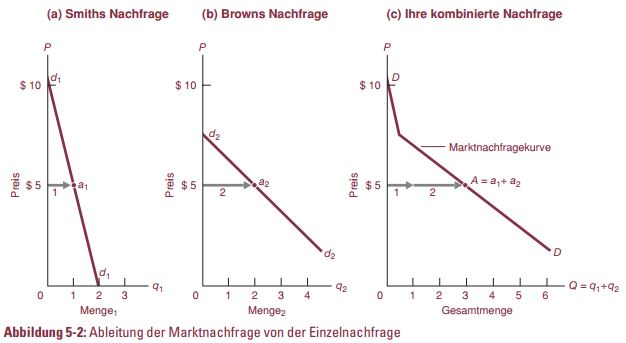
\includegraphics[width=0.48\textwidth]{img/kombinierte-nachfrage.jpg}
  \end{center}
  \vspace{-20pt}
\end{wrapfigure}
Die Marktnachfragekurve ist die Summe der Einzelnachfragen zu jedem Preis. Abbildung 5-2 zeigt, wie die einzelnen Nachfragekurven dd horizontal zu addieren sind, um die 
Marktnachfragekurve DD zu erhalten. \\ \\ \\ \\ \\
\subsubsection{Güterklassifizerung}
\begin{itemize}
\item Güter sind {\bf Substitute}, wenn eine Preiserhöhung bei einem Gut die Nachfrage nach dem anderen verstärkt.
\item Güter sind {\bf Ergänzungsprodukte}, wenn eine Preiserhöhung bei einem Gut die Nachfrage nach dem anderen senkt.
\item Güter sind {\bf unabhängig}, wenn eine Preisänderung bei einem Gut keine Auswirkungen auf die Nachfrage nach dem anderen Gut hat. 
\end{itemize}
\subsubsection{Beispiel: Suchtmittel Nachfrage}
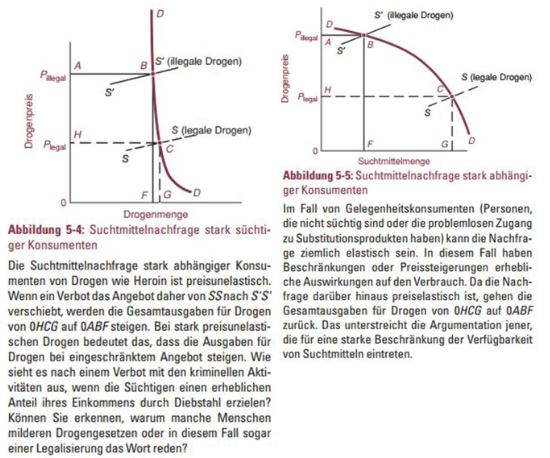
\includegraphics[width=0.6\textwidth]{img/junkies.jpg}
\newpage
\subsection{Konsumrente}
\begin{wrapfigure}{l}{0.3\textwidth}
\vspace{-20pt}
  \begin{center}
    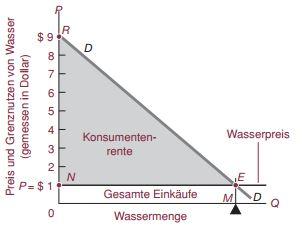
\includegraphics[width=0.28\textwidth]{img/konsumrente.jpg}
  \end{center}
  \vspace{-20pt}
\end{wrapfigure}
Da die Konsumenten für alle konsumierten Einheiten nur den Preis der letzten Einheit bezahlen, erzielen sie einen Nutzengewinn gegenüber den Kosten. Die Konsumentenrente entspricht dem zusätzlichen Wert, den die Konsumenten gegenüber dem Preis erzielen, den sie für ein Wirtschaftsgut bezahlt haben.\\
{\it Bild: Die Nachfragekurve misst, wie viel die Konsumenten freiwillig für jede konsumierte Einheit bezahlen würden. Daher zeigt der gesamte Bereich unter der Nachfragekurve (0REM) den Gesamtnutzen aus dem Konsum von Wasser. Indem man die Marktkosten des Wassers für die Konsumenten (entsprechend 0NEM) subtrahiert, erhält man die Konsumentenrente aus dem Wasserkonsum in Form des grauen Dreiecks NER. Diese Methode ist für die Messung des Nutzens öffentlicher Güter und der Verluste aus Monopolen und Importzöllen überaus nützlich.}


\section{Produktion und ihre Organisation im Unternehmen}
\subsection{Grundlagen}
\subsubsection{Produktionsfunktion}
Die Produktionsfunktion sagt aus, welche maximale Produktionsmenge bei gegebenem Faktoreinsatz erzeugt werden kann. Sie gilt jeweils für einen bestimmten Stand der Technik und des technologischen Know-hows. 
\subsubsection{Gesamt-, Durchschnitts- und Grenzprodukt}
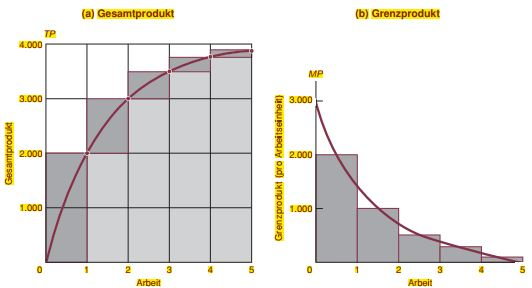
\includegraphics[width=0.48\textwidth]{img/grenzprodukt.jpg}
{\bf Gesamtprodukt}, die Gesamtanzahl der produzierten Outputs in physischen Einheiten (Tuben bei Zahnpasta). Das {\bf Grenzprodukt } oder die Grenzproduktivität eines Inputs oder Produktionsfaktors entspricht der zusätzlichen Menge oder dem zusätzlichen Output, die bzw. der durch eine zusätzliche Einheit erzeugt werden kann, während alle anderen Faktoren konstant bleiben. {\bf Durchschnittsprodukt}, der Gesamtoutput dividiert durch die gesamten Inputeinheiten.
\subsubsection{Das Gesetz der abnehmenden Grenzerträge (Ertragsgesetz)}
Das Ertragsgesetz besagt, dass wir laufend geringere zusätzliche Erträge erhalten, wenn wir einen Input bei unveränderten sonstigen Faktoren immer weiter erhöhen. Mit anderen Worten, das Grenzprodukt jeder Inputeinheit sinkt, wenn sich die Menge dieses Inputs erhöht, während alle anderen Faktor konstant bleiben.\\
\\
{\it Das Ertragsgesetz ist eher eine weithin beobachtete empirische Gesetzmäßigkeit als eine universelle Wahrheit, wie wir sie etwa dem Gesetz der Schwerkraft zubilligen.}
\subsection{Skalenerträge}
Die Produktion zeigt konstante, abnehmende oder zunehmende Skalenerträge, je nachdem ob eine gleichmäßige Erhöhung aller Faktoren zu einem überproportionalen, unterproportionalen oder proportionalen Anstieg der Produktionsmenge führt.\begin{itemize}
\item {\bf Konstante Skalenerträge} liegen vor, wenn eine Änderung aller Inputs zu einer Veränderung des Outputs im selben Verhältnis führt. 
\item {\bf Zunehmende Skalenerträge} treten ein, wenn eine Erhöhung aller Inputs zu einem überproportionalen Anstieg des Outputs führt. 
\item {\bf Abnehmende Skalenerträge } treten auf, wenn eine gleichmäßige Erhöhung aller Inputs zu einer unterproportionalen Erhöhung des Gesamtoutputs führt.
 \end{itemize}

\subsection{Kurzfristige und Langfristige Betrachtungsweise}
Für eine effiziente Produktion sind sowohl Zeit als auch konventionelle Produktionsfaktoren wie Arbeit erforderlich. Wir unterscheiden daher in Produktion und Kostenanalyse zwischen zwei unterschiedlich langen Zeitperioden. Als {\bf kurzfristig} wird dabei ein Zeitraum betrachtet, innerhalb dessen nur einige, nämlich die {\it variablen Faktoreinsätze} angepasst werden können. Fixe Faktoren wie Anlagen und Ausstattung lassen sich dagegen kurzfristig nicht vollständig ändern oder anpassen. Als  {\bf langfristig} wird ein Zeitraum bezeichnet, in dem alle fixen und variablen Faktoren, derer sich das Unternehmen bedient, einschließlich Kapital, verändert werden können.

\subsection{Technologischer Wandel}
Wir unterscheiden zwischen {\bf Prozessinnovation} , die dann gegeben ist, wenn neues technisches Know-how die Produktionstechnik für bestehende Produkte verbessert, und {\bf Produktinnovation}, wenn neue oder verbesserte Produkte auf den Markt gebracht werden.  

\subsection{Produktivität und aggregierte Produktionsfunktion}
\subsubsection{Produktivität}
{\bf Produktivität} ist ein Konzept zur Messung des Verhältnisses zwischen dem Gesamtoutput und einem gewichteten Inputdurchschnitt. Zwei bedeutende Varianten der Produktivität sind die {\bf Arbeitsproduktivität}, die den Output je Arbeitseinheit errechnet und die {\bf Gesamtfaktorproduktivität}, die den Output je Einheit der Gesamtinputs misst (typischerweise bestehend aus Kapital und Arbeit).
\subsubsection{Produktivitätswachstum durch Skaleneffekte}
Die Produktivität wächst aufgrund von Skaleneffekten und technologischem Fortschritt. Skaleneffekte und Massenproduktion waren im vergangenen Jahrhundert bedeutende Produktivitätsfaktoren. Die meisten Produktionsprozesse sind heute sehr viel umfangreicher als im 19. Jahrhundert. Ein großes Schiff konnte um die Mitte des 19. Jahrhunderts 2.000 Tonnen Güter befördern, während die heutigen Supertanker mehr als 1 Million Tonnen Öl laden und befördern. 
\subsection{Unternehmen}
Unternehmen sind spezialisierte Gebilde, die sich mit dem Management des Produktionsprozesses befassen. Die Produktion wird deshalb in Unternehmen organisiert, weil Effizienz im Regelfall Produktion im großen Maßstab, die Beschaffung erheblicherfinanzieller Mittel und die Überwachung des laufenden Betriebs erfordert.
\subsubsection{Einzelfirma}
Am unteren Ende des Spektrums befindet sich die Einzelfirma, der klassische Kleinbetrieb, den wir alle kennen. In einem kleinen Laden werden vielleicht ein paar hundert Dollar täglich umgesetzt, und er ernährt seinen Besitzer nur mit Mühe.
\subsubsection{Personengesellschaft}
Ein Unternehmen verlangt häufig nach einer entsprechenden Kombination von Fähigkeiten – etwa nach Rechtsanwälten oder Ärzten, die sich auf unterschiedlichen Gebieten spezialisiert haben. Tun sich zwei oder mehr Personen zusammen, können sie eine Personengesellschaft gründen. diese Unternehmensform bringt bestimmte Nachteile mit sich, die sie für Großbetriebe ungeeignet macht. Ihr Hauptnachteil ist die unbeschränkte Haftung.
\subsubsection{Kapitalgesellschaft}
\begin{itemize}
\item Das Eigentum an der Kapitalgesellschaft ergibt sich aus dem Eigentum an den Stammaktien der Gesellschaft.
\item Im Prinzip kontrollieren die Aktionäre die Kapitalgesellschaften, die sich in ihrem Eigentum befinden.
\item Die Vorstände und Aufsichtsräte der Kapitalgesellschaften sind rechtlich befugt, Entscheidungen für die Gesellschaft zu treffen.
\end{itemize}
Eine effiziente Produktion erfordert häufig große Unternehmenseinheiten, die Kapitalinvestitionen in Milliardenhöhe benötigen. Kapitalgesellschaften mit ihrer beschränkten Haftung und praktischen Managementstruktur können sehr viel privates Kapital anziehen, eine ganze Palette verwandter Güter produzieren und auch das Anlegerrisiko auf viele Schultern verteilen. 

\section{Kostenanalyse}
\subsection{Gesamtkosten: Fixkosten und variable Kosten}
{\bf Gesamtkosten } stellen die in Geld ausgedrückten Mindestgesamtausgaben dar, die benötigt werden, um eine bestimmte Produktionsmengeq zu erzielen. Die {\it Gesamtkosten TC}  steigen, sobald q steigt. \\
{\bf Fixkosten } stellen den gesamten, in Geld ausgedrückten Ausgabenbetrag dar, der selbst dann aufgewendet werden muss, wenn keine Produktionsleistung erzielt wird. Fixkosten bleiben durch Änderungen der Produktionsmenge unbeeinflusst.\\
{\bf Variable Kosten } sind Ausgaben, die mit der Produktionsmenge variieren. Dazu gehören Rohmaterialien, Löhne und Treibstoffe, eben alle Kosten, die keine Fixkosten sind. \\
Per definitionem gilt daher immer:
\begin{equation}
TC = FC + VC \nonumber
\end{equation}
\subsection{Grenzkosten}
\begin{wrapfigure}{l}{0.3\textwidth}
\vspace{-20pt}
  \begin{center}
    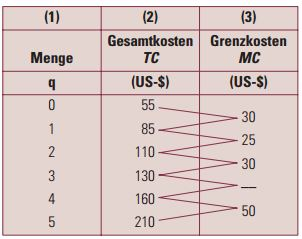
\includegraphics[width=0.28\textwidth]{img/grenzkosten_einfach.jpg}
  \end{center}
  \vspace{-20pt}
\end{wrapfigure}
Die Grenzkosten sind eines der zentralen volkswirtschaftlichen Konzepte. Mit diesem Begriff, Grenzkosten (MC), werden alle zusätzlichen Kosten bezeichnet, die bei der Erzeugung jeweils einer zusätzlichen Produktionseinheit anfallen. Produziert ein Unternehmen beispielsweise 1.000 CDs zu Gesamtkosten von US-\$ 10.000 und kostet es US-\$ 10.006, eine mehr, nämlich 1.001 CDs herzustellen, so liegen die Grenzkosten für die Produktion der 1.001. CD bei US-\$ 6.\\ \\
\subsubsection{Grenzkosten im Diagramm}
\begin{wrapfigure}{l}{0.5\textwidth}
\vspace{-20pt}
  \begin{center}
    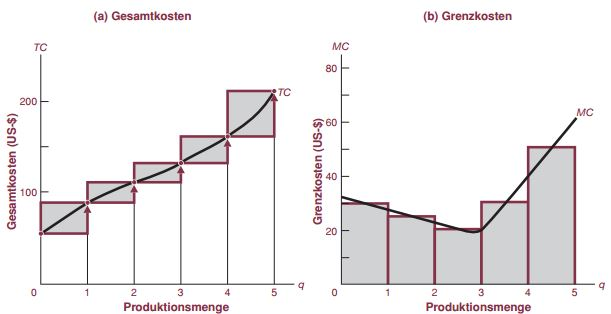
\includegraphics[width=0.48\textwidth]{img/grenzkosten_diagramm.jpg}
  \end{center}
  \vspace{-10pt}
\end{wrapfigure}
In der vorliegenden Abbildung sind die Daten aus Tabelle 7-2 im Diagramm dargestellt. Die Grenzkosten in (b) werden berechnet, indem man die Zusatzkosten, die laut (a) für jede zusätzliche Produktionseinheit anfallen, feststellt. Um daher die Produktions-MCfür die fünfte Einheit ermitteln zu können, subtrahieren wir US-\$ 160 von US-\$ 210 und erhalten MC = US-\$ 50. Eine durchgängige schwarze Kurve wurde in (a) durch die einzelnen TC-Punkte gezogen, und eine durchgängige schwarze Kurve verbindet auch in (b) die unterschiedlichen MC-Stufen.\\ \\
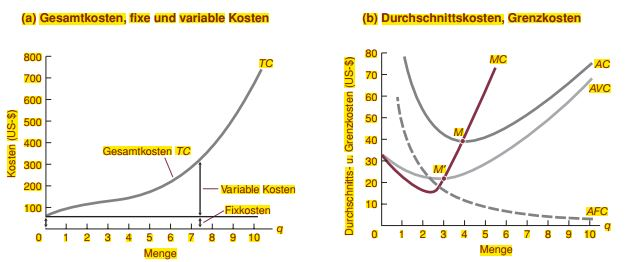
\includegraphics[width=0.68\textwidth]{img/gesamtkosten.jpg}
\begin{itemize}
\item Die Gesamtkosten setzen sich aus fixen und variablen Kosten zusammen.
\item Die rote Grenzkostenkurve fällt erst ab und steigt dann wieder an, wie durch die MC-Daten in Spalte (5) der Tabelle weiter unten angegeben. Bitte beachten Sie, dass MC die AC-Kurve in ihrem Minimum schneidet.
\end{itemize}

\subsection{Durchschnittskosten}
{\bf Durchschnittskosten} sind die Gesamtkosten, dividiert durch die Gesamtanzahl der produzierten Einheiten. Daher gilt:\\
\begin{equation}
\text{Durchschnittskosten} = \frac{\text{Gesamtkosten}}{\text{Produktionsmenge}} = \frac{TC}{q} = AC \nonumber
\end{equation}
\subsection{Weitere Kostendefinitionen}
\begin{itemize}
\item {\bf Durschnittsfixkosten}
\begin{equation}
AFC = \frac{FC}{q} \nonumber
\end{equation}
\item {\bf durchschnittliche variable Kosten}
\begin{equation}
AVC = \frac{VC}{q} \nonumber
\end{equation}
\end{itemize}
\newpage
\subsubsection{Tabelle}
\begin{wrapfigure}{l}{0.5\textwidth}
\vspace{-20pt}
  \begin{center}
    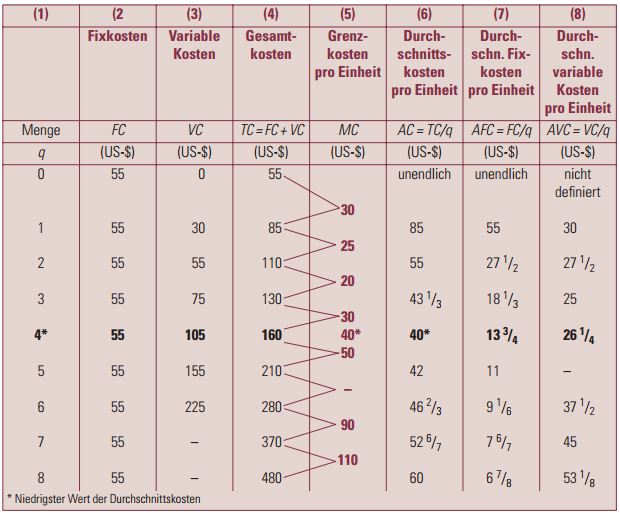
\includegraphics[width=0.48\textwidth]{img/kosten.jpg}
  \end{center}
  \vspace{-20pt}
\end{wrapfigure}
Wenn die Grenzkosten unter den Durchschnittskosten liegen, senken Sie die Durchschnittskosten.\\
Wenn die MC über den AC liegen, erhöhen Sie die AC.\\
Wenn die MC genau den AC entsprechen, fallen oder steigen die AC in diesem Punktnicht und befinden sich auf ihrem Mindestniveau. Daher gilt am tiefsten Wert einer U-förmigen AC-Kurve: MC = AC = geringstmögliche AC.\\ \\ \\ \\  \\ \\ 
\subsection{Abnehmende Erträge und U-förmige Kostenkurven}
\begin{itemize}
\item
{\bf Kurzfristig } bedeutet einen Zeitraum, der lang genug ist, um die variablen Produktionsfaktoren wie Material und Arbeit anzupassen, jedoch zu kurz, um alle Produktionsfaktoren variieren zu können. Kurzfristig können fixe oder Overhead-Faktoren wie Anlagen und Betriebsausstattung nicht vollständig verändert oder angepasst werden. Deshalb sind die Arbeits- und Materialkosten im Normalfall variable Kosten, während die Kapitalkosten zu den Fixkosten gehören.
\item {\bf Langfristig} lassen sich alle Inputs anpassen – Arbeit ebenso wie Rohstoffe und Kapital. Langfristig sind daher alle Kosten variabel und nicht fix. 
\end{itemize}
Kurzfristig, wenn bestimmte Faktoren wie das Kapital fix sind, weisen die variablen Faktoren eine erste Phase steigender Grenzerträge auf, worauf eine Phase abnehmender Erträge folgt. Die entsprechenden Kostenkurven zeigen eine erste Phase abnehmender Grenzkosten, worauf eine Phase steigender Grenzkosten folgt, sobald die Grenzerträge sinken.\\ \\
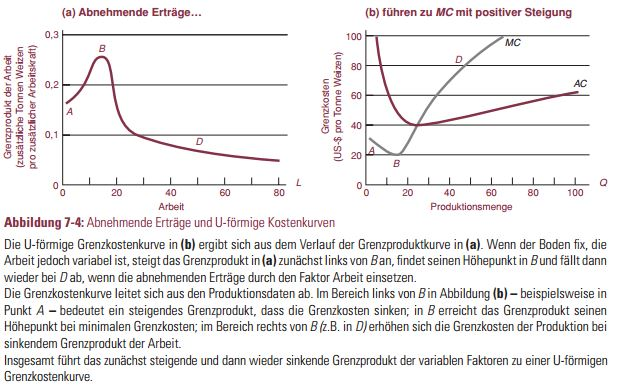
\includegraphics[width=0.88\textwidth]{img/ertrage.jpg}
\subsection{Least-Cost-Regel}
Um eine bestimmte Produktionsleistung mit den geringstmöglichen Kosten erzielen zu können, muss ein Unternehmen bei der Beschaffung der Produktionsfaktoren darauf achten, dass das Grenzprodukt pro Geldeinheit, die für jeden einzelnen Produktionsfaktor ausgegeben wird, gleich hoch ist. Das heißt: (siehe Abb. 7-4 für A,L)\\
\begin{equation}
\frac{\text{Grenzpunkt von L}}{\text{Preis von L}} = \frac{\text{Grenzpunkt von A}}{\text{Preis von A}}  \nonumber
\end{equation}
\subsection{Substitutionsregel}
Wenn der Preis für einen Produktionsfaktor sinkt, während alle anderen Faktorpreise gleich bleiben, profitiert ein Unternehmen davon, den verbilligten Faktor anstelle der sonstigen Optionen einzusetzen.


\subsection{Volkswirtschaftliche und betriebswirtschaftliche Kostenrechnung}
\begin{equation}
\textbf{Nettoertrag} = \text{Gesamterlös - Gesamtaufwand} \nonumber
\end{equation}
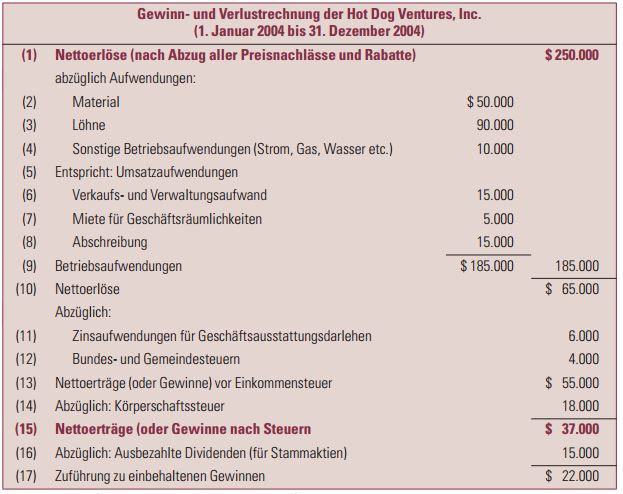
\includegraphics[width=0.5\textwidth]{img/kostenrechnung.jpg}
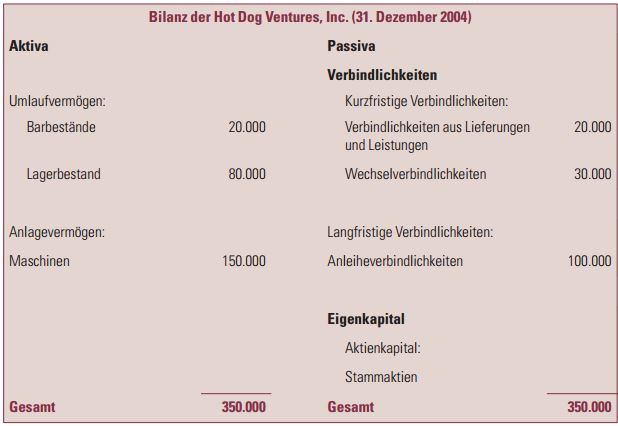
\includegraphics[width=0.5\textwidth]{img/bilanz.jpg}
{\bf Unterschied Bilanz und Gewinn/Verlustrechnung}\\
Die Gewinn- und Verlustrechnung misst die Ströme {\it Flussgrösse} in ein Unternehmen hinein und aus ihm heraus, während die Bilanz den Bestand {\it Bestandsgrösse}  an Aktiva und Passiva zum Ende eines Geschäftsjahres darstellt.
\begin{itemize}
\item[1] Verkaufserlöse {Punkt 1}
\item[2] Aufwendungen {Punkte 2-8}
\item[3] Nettoerträge {Punkte 15}
\end{itemize}
\subsubsection{Begriffserläuterungen}
Die {\bf Abschreibung} ist ein Maß für die jährlichen Kosten eines Kapital-Inputs, den ein Unternehmen selbst besitzt. Dieselbe Überlegung gilt für sämtliche Kapitalgüter eines Unternehmens.\\
Formeln zur Berechnung der jährlichen Abschreibung, aber sie alle folgen zwei wichtigen Prinzipien:\\ (a) Die Abschreibung des betreffenden Wertes muss den historischen Kosten oder dem Anschaffungspreis entsprechen;\\ (b) die Abschreibung wird während der buchhalterischen Nutzungsdauer, die sich an der tatsächlichen Nutzungsdauer orientiert, in Form jährlicher Aufwendungen verbucht. \\ 
\\
So gehört zum betrieblichen Rechnungswesen auch die {\bf Bilanz }, die ein Bild von der jeweiligen finanziellen Situation eines Unternehmens zu einem bestimmten Zeitpunkt zeichnet.\\
Auf der einen Seite der Bilanz stehen die {\bf Aktiva} (Vermögenswerte und Rechte des Unternehmens). Auf der anderen, der Passivseite, finden sich zwei Positionen, nämlich die {\bf Verbindlichkeiten }(Schulden und sonstige Verpflichtungen des Unternehmens) und das {\bf Eigenkapital }(der Nettowert, der den Gesamtvermögenswerten abzüglich der gesamten Verbindlichkeiten entspricht).\\
Die wichtigste Annahme, die jeder Bilanz zugrunde gelegt wird, lautet, dass der Wert beinahe jeder Position deren Anschaffungskosten (historischen Kosten) entspricht. \\
\begin{equation}
\text{Gesamtvermögenswerte (Aktiva)} = \text{Gesamtverbindlichkeiten + Eigenkapital} \nonumber
\end{equation}
\begin{equation}
\text{Eigentkapital} = \text{Vermögen (Aktiva) - Verbindlichkeiten} \nonumber
\end{equation}
\subsection{Opportunitätskosten}
Beim Treffen von Entscheidungen fallen Opportunitätskosten an, weil die Auswahl einer Möglichkeit in einer Welt der Knappheit bedeutet, dass wir auf andere Möglichkeiten verzichten müssen. Opportunitätskosten bezeichnen den Wert des wertvollsten entgangenen Gutes oder der entgangenen Dienstleistung.\\
Die volkswirtschaftlichen Kosten berücksichtigen zusätzlich zu den tatsächlichen Geldausgaben alle Opportunitätskosten, die entstehen, weil Ressourcen auch anderweitig eingesetzt werden könnten. \\
{\it Auf gut funktionierenden Märkten entsprechen die Preise den Opportunitätskosten. }
\section{Analyse des Marktes bei vollkommenem Wettbewerb, also nie...}
\subsection{Angebotsverhalten von Unternehmen}
\begin{wrapfigure}{l}{0.3\textwidth}
  \begin{center}
    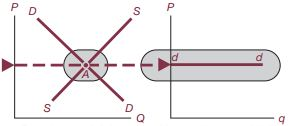
\includegraphics[width=0.28\textwidth]{img/nachfrage_voll_wett.jpg}
  \end{center}
\end{wrapfigure}
Der vollständige Wettbewerb ist eine Welt der Preisnehmer. Ein im vollständigen Wettbewerb stehendes Unternehmen verkauft ein homogenes Produkt (eines, das mit dem von anderen Branchenteilnehmern verkauften Produkt identisch ist). Das Unternehmen ist im Vergleich zu seinem Markt so klein, dass es keinen Einfluss auf den Marktpreis nehmen kann; es betrachtet den Preis daher als eine gegebene Größe.\\
Da ein Wirtschaftszweig unter Wettbewerbsbedingungen von Unternehmen bevölkert wird, die gemessen am Gesamtmarkt klein sind, entspricht die Nachfragekurve dieses Unternehmens nur einem winzigen Segment der Nachfragekurve der Gesamtbranche. Grafisch dargestellt ist der Anteil des einzelnen Unternehmens an der Nachfragekurve so gering, dass aus der Froschperspektive des Marktteilnehmers im vollständigen Wettbewerb die Nachfragekurve dd absolut horizontal und unbegrenzt elastisch erscheint.\\
\begin{itemize}
\item Unter den Bedingungen des vollständigen Wettbewerbs gibt es zahlreiche kleine Unternehmen, die ein identisches Produkt erzeugen und jeweils zu klein sind, um auf den Marktpreis Einfluss zu nehmen. 
\item Für das Unternehmen im vollständigen Wettbewerb gilt eine völlig waagrechte Nachfragekurve.
\item Der zusätzliche Erlös aus jeder zusätzlich verkauften Einheit entspricht daher dem Marktpreis.
\end{itemize} 
\subsubsection{Angebot unter Wettbewerbsbedingungen}
\begin{wrapfigure}{l}{0.5\textwidth}
  \begin{center}
   \vspace{-20pt}
    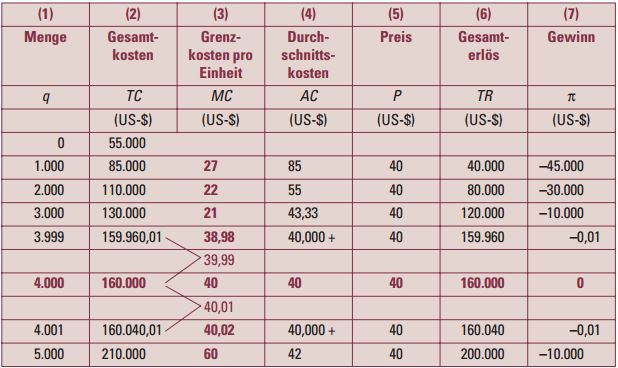
\includegraphics[width=0.48\textwidth]{img/hans.jpg}
      \vspace{-20pt}
  \end{center}
\end{wrapfigure}
Der maximale Gewinn ergibt sich bei jener Produktionsmenge, bei der die Grenzkosten dem Preis entsprechen. \\
Regel für die Angebotsmenge eines Unternehmens unter den Bedingungen vollständigen Wettbewerbs: Ein Unternehmen, das nach Gewinnmaximierung strebt, wählt eine Produktionsmenge, bei der die Grenzkosten dem Preis entsprechen:\\
Grenzkosten = Preis oder MC = P\\
Im Allgemeinen kann ein Unternehmen mithilfe seiner Grenzkostenkurve seine optimale Produktionsmenge ermitteln: Die Gewinnmaximierung wird bei jener Produktionsmenge erreicht, bei der Preis- und Grenzkostenkurve einander schneiden.
\subsubsection{Break-Even-Punkt}
Beschreibt jene Produktionsmenge, bei der das Unternehmen einen Gewinn von Null erzielt. Im Break-even-Punkt entspricht der Preis den Durchschnittskosten, daher decken die Erlö- se gerade die Kosten ab.  

\subsubsection{Gewinnmaximierung - allgemein}
Ein Unternehmen, das auf Gewinnmaximierung bedacht ist, entscheidet sich für jene Produktionsmenge, bei der die Grenzkosten dem Preis entsprechen. Im Diagramm bedeutet das, dass die Grenzkostenkurve eines Unternehmens seiner Angebotskurve entspricht.\\
\begin{wrapfigure}{r}{0.3\textwidth}
  \begin{center}
    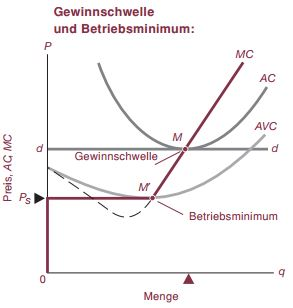
\includegraphics[width=0.28\textwidth]{img/betriebsminimum.jpg}
    \vspace{-20pt}
    \end{center}
\end{wrapfigure}
\subsubsection{Betriebsminimum}
Die kritische Marktpreisuntergrenze, bei der die Erlöse genau den variablen Kosten entsprechen (oder bei der die Verluste genau den Fixkosten entsprechen), wird als Betriebsminimum bezeichnet.
\subsubsection{Betriebseinstellungsregel}
 Das Betriebsminimum ist der Punkt, an dem die Erlöse die variablen Kosten gerade abdecken oder an dem die Verluste den Fixkosten entsprechen. Wenn der Preis so weit fällt, dass der Preis geringer ist als die durchschnittlichen variablen Kosten, kann das Unternehmen durch Betriebseinstellung seine Gewinne maximieren (seine Verluste minimieren).\\
 \\
Graphik: {\it Die Angebotskurve des Unternehmens entspricht seiner MC-Kurve, solange der Erlös höher ist als die variablen Kosten. Sobald der Preis unter das Betriebsminimum Ps fällt, übersteigen die Verluste die Fixkosten, und das Unternehmen stellt die Produktion ein. Daher stellt die durchgängige rostfarbene Kurve die Angebotskurve des Unternehmens dar.}

\subsection{Das Angebotsverhalten ganzer Wirtschaftszweige}
Um die Marktangebotskurve für ein Gut zu ermitteln, müssen wir die Angebotskurven aller einzelnen Produzenten dieses Gutes horizontal addieren.Die horizontale Addition der Produktionsmengen beim jeweiligen Preis ergibt die Branchen-Angebotskurve.

\begin{wrapfigure}{r}{0.4\textwidth}
  \begin{center}
  	\vspace{-20pt}
    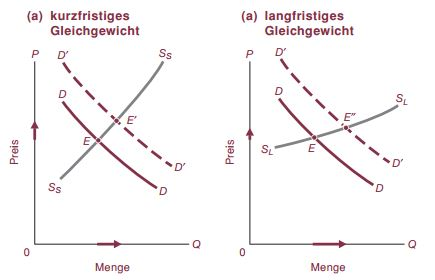
\includegraphics[width=0.38\textwidth]{img/marshall.jpg}
    \vspace{-20pt}
    \end{center}
\end{wrapfigure}
Wir unterscheiden zwischen (a) Perioden, in denen die Unternehmen nur für Anpassungen beim Einsatz des Faktors Arbeit und der anderen variablen Faktoren genügend Zeit haben (kurzfristiges Gleichgewicht) und (b) Perioden, in denen die vollständige Anpassung des Einsatzes der Faktoren – und zwar der fixen wie der variablen – möglich ist (langfristiges Gleichgewicht). Je mehr Zeit für Anpassungen zur Verfügung steht, desto  größer fällt die Elastizität der Angebotsreaktion und desto geringer die Preissteigerung aus. 

\subsubsection{Addition von Angebotskurven}
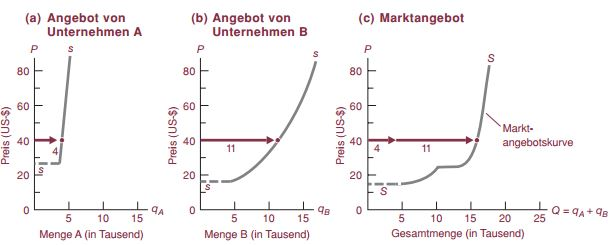
\includegraphics[width=0.98\textwidth]{img/addition.jpg}
\subsubsection{Langfristiges Break-even-Gleichgewicht}
Bei einer im Wettbewerb stehenden Branche mit identischen, frei in den Markt ein- und austretenden Unternehmen lautet die langfristige Gleichgewichtsbedingung wie folgt: Für jedes identische Unternehmen entspricht der Preis den Grenzkosten sowie den langfristigen Mindest-Durchschnittskosten: \\
P = MC = minimale langfristige AC = Breakeven-Preis\\
Dies ist die Bedingung, unter der der Gewinn langfristig gegen null tendiert („zero-economic-profit“).
Was die langfristige Rentabilität des wettbewerbsorientierten Kapitalismus anbelangt,
kommen wir zu einem überraschenden Schluss. Wir stellen fest, dass die Wettbewerbskräfte die Unternehmen langfristig in Richtung Gewinnschwelle treiben. Auf lange Sicht erzielen im Wettbewerb stehende Unternehmen eine normale Rendite auf ihre Investitionen, aber nicht mehr. Gewinnträchtige Wirtschaftszweige ziehen neue Unternehmen an, was zu Preissenkungen und niedrigeren Gewinnen führt, bis sich die Gewinne gegen null bewegen. Im Gegensatz dazu streben Unternehmen in nicht gewinnträchtigen Branchen nach besseren Renditechancen in anderen Wirtschaftszweigen; Preise und Gewinne tendieren daraufhin nach oben. Im langfristigen Gleichgewicht einer im Wettbewerb stehenden Branche wird daher kein Gewinn erzielt.
\subsection{Allgemeine Regeln}
\subsubsection{Nachfrageregel}
In aller Regel treibt eine Erhöhung der Nachfrage nach einem Gut bei unveränderter Angebotskurve den Preis dieses Gutes in die Höhe. Bei den meisten Gütern bewirkt eine erhöhte Nachfrage auch eine Erhöhung der nachgefragten Menge. Ein Rückgang der Nachfrage hat die gegenteilige Wirkung.
\subsubsection{Angebotsregel}
Ein vermehrtes Angebot eines Gutes (bei konstanter Nachfragekurve) führt im Allgemeinen zu einer Preissenkung und einer Erhöhung der Kauf- und Verkaufsmenge. Ein Angebotsrückgang hat den gegenteiligen Effekt.\\
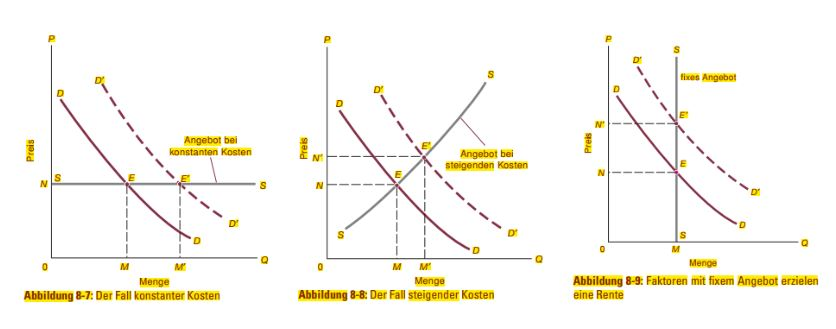
\includegraphics[width=0.88\textwidth]{img/kostenarten.jpg}
\subsubsection{Angebotsverschiebungen}
\begin{itemize}
\item  Ein vermehrtes Angebot senkt P dann am stärksten, wenn die Nachfrage unelastisch ist. 
\item Ein vermehrtes Angebot erhöht Q dann am wenigsten, wenn die Nachfrage unelastisch ist.
\end{itemize}
\subsection{Effizienz und Verteilungsgerechtigkeit auf Wettbewerbsmärkten}
\subsubsection{Effizienzkonzept}
Von {\bf Allokationseffizienz }(oder Effizienz) kann man sprechen, wenn niemand durch eine andere Organisation der Produktion besser gestellt werden kann, ohne dass dadurch zugleich jemand anderer schlechter gestellt wird. Unter den Bedingungen allokativer Effizienz lässt sich eine Steigerung der Bedürfnisbefriedigung oder des Nutzens für eine Person nur durch Schmälerung des Nutzens für eine andere Person erreichen. 

\subsubsection{wirtschaftliche Rente}
\begin{wrapfigure}{r}{0.4\textwidth}
  \begin{center}
  	\vspace{-20pt}
    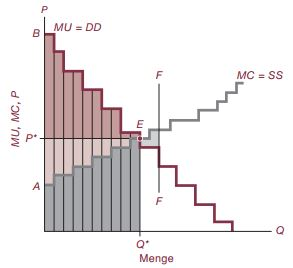
\includegraphics[width=0.38\textwidth]{img/allokation.jpg}
    \vspace{-20pt}
    \end{center}
\end{wrapfigure}
Die Abbildung zeigt ein neues Konzept, die wirtschaftliche Rente, die als rostfarbener Bereich zwischen den Angebots- und Nachfragekurven im Gleichgewicht dargestellt ist. Die 
wirtschaftliche Rente ist die Summe der im 5. Kapitel beschriebenen Konsumentenrente – des Bereichs zwischen der Nachfragekurve und der Preislinie – und der Produzentenrente – des Bereichs zwischen der Preislinie und der SS-Kurve. Die Produzentenrente beinhaltet die Renten und Gewinne von Firmen und Eigentümern spezialisierter, in der Branche eingesetzter Inputs und gibt den Überschluss der Erträge gegenüber den Produktionskosten an. Die volkswirtschaftliche Rente drückt den aus Produktion und Konsum eines Gutes zusätzlich gewonnenen Nettonutzen oder Wohlstand aus. Sie entspricht der Konsumentenrente plus der Produzentenrente .\\
\\
Eine weitere Möglichkeit, die Effizienz des Wettbewerbsgleichgewichts zu betrachten, ist er Vergleich der wirtschaftlichen Auswirkungen einer kleinen Änderung des Gleichgewichts bei E. Wie der folgende Dreistufenprozess zeigt, ist die Allokation effizient, wenn MU = P = MC.
\begin{itemize}
\item P = MU. Die Konsumenten entscheiden sich für den Kauf von Nahrungsmitteln bis zu jenem Betrag, bei dem gilt: P = MU. Folglich gewinnt jede Person aus der letzten konsumierten Nahrungsmitteleinheit P Nutzeneinheiten oder Utils.
\item P = MC. Als Produzent bietet jede der Personen aus unserem Beispiel Nahrungsmittel bis zu dem Punkt an, an dem der Nahrungsmittelpreis genau den MC der letzten angebotenen Nahrungsmitteleinheit entspricht (wobei hier die MC die Kosten des Freizeitverzichts sind, der zur Produktion der letzten Nahrungsmitteleinheit erforderlich ist). Der Preis entspricht daher den Freizeit-Utils, auf die für die Produktion dieser letzten Nahrungsmitteleinheit verzichtet werden muss.
\item Wenn wir diese beiden Gleichungen zusammenfügen, erkennen wir, dass MU = MC.
Das bedeutet, dass die durch die letzte konsumierte Nahrungsmitteleinheit gewonnenen Nutzeneinheiten exakt den durch den Zeitaufwand für die Produktion dieser letzten produzierten Nahrungsmitteleinheit verlorenen Freizeit-Utils entsprechen. Und genau diese Bedingung, wonach der Grenzgewinn aus der letzten konsumierten Einheit genau den Grenzkosten der Gesellschaft für die letzte produzierte Einheit entspricht, ist es, die uns garantiert, dass ein Wettbewerbsgleichgewicht effizient ist.
\end{itemize}
WICHTIG:\\
Der vollkommene Markt ist ein Instrument zur Verbindung (a) der Bereitschaft der Konsumenten mit entsprechender Kaufkraft, für Güter zu bezahlen, mit (b) den Grenzkosten dieser Güter, die durch das Angebot der Unternehmen repräsentiert werden. Unter bestimmten Bedingungen garantiert der Wettbewerb Effizienz, was bedeutet, dass kein zusätzlicher Nutzen eines Konsumenten erzielbar ist, ohne zugleich den Nutzen eines anderen Konsumenten zu schmälern. Das trifft auch in einer Welt mit unzähligen Produktionsfaktoren und Produkten zu.\\
{\bf Die tragende Rolle der Grenzkosten in einer Marktwirtschaft erklärt sich wie folgt: Nur wenn die Preise den Grenzkosten entsprechen, holt diese Wirtschaft den maximalen Output und die größtmögliche Bedürfnisbe-friedigung aus ihren knappen Ressourcen an Grund und Boden, Arbeit und Kapital heraus. } 


\section{Unvollständiger Wettbewerb und Monopol}
{\bf Unvollständiger Wettbewerb } herrscht in einem Wirtschaftszweig immer dann, wenn einzelne Anbieter ein gewisses Maß an Kontrolle über den Preis ihrer Produkte ausüben.\\
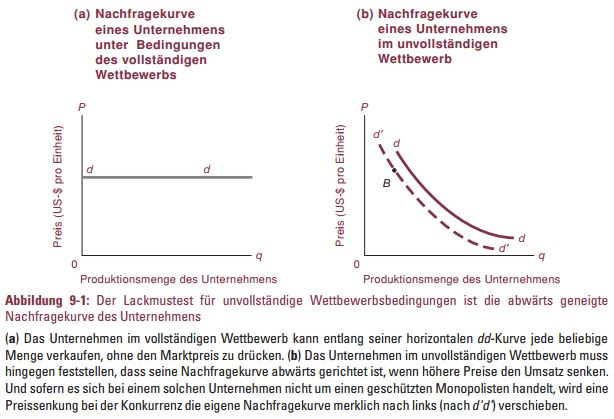
\includegraphics[width=0.88\textwidth]{img/unvollstandig.jpg}
\subsection{Die Formen des unvollständigen Wettbewerbs}
\subsubsection{Marktstrukteren}
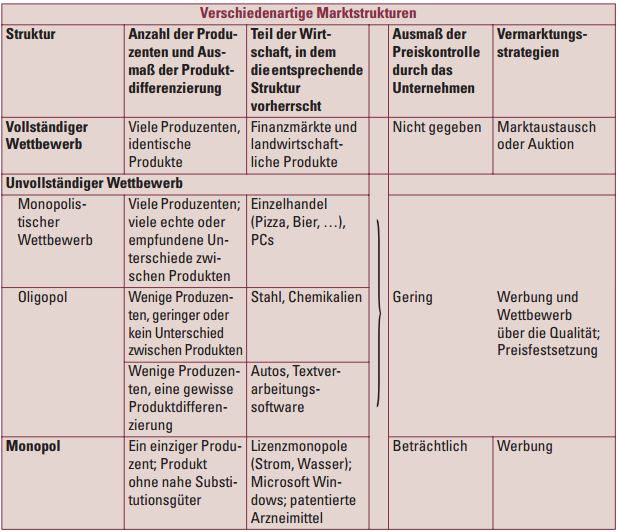
\includegraphics[width=0.98\textwidth]{img/wettbewerb.jpg}

\subsubsection{Ursachen für die Unvollkommenheit des Marktes}
Die meisten Fälle unvollständigen Wettbewerbs lassen sich auf zwei wesentliche Gründe zurückführen.
\begin{itemize}
\item[] Erstens gibt es in einem Wirtschaftszweig tendenziell weniger Anbieter, wenn Skaleneffekte und eine damit einhergehende Kostensenkung in der Produktion eine besondere Bedeutung haben. Unter diesen Bedingungen können große Unternehmen einfach billiger produzieren und damit die Kleinen unterbieten, die das häufig nicht überleben.
\item[] Zweitens tendieren Märkte zum unvollständigen Wettbewerb, wenn neue Mitbewerber „Zutrittsbarrieren“ überwinden müssen.
\end{itemize}
\subsubsection{Kosten und Marktunvollkommenheit}
Die entscheidende Frage lautet, welche Bedeutung Skaleneffekte in einem bestimmten Wirtschaftszweig haben. Wenn Skaleneffekte eine wichtige Rolle spielen, werden ein oder mehrere Unternehmen ihre Produktion bis auf ein Niveau erhöhen, bei dem sie schließlich den Großteil der Gesamtproduktionsmenge herstellen. Doch unabhängig davon, wie sich die Branchenstruktur auf Grund von Skaleneffekten darstellt, werden wir in jedem Fall eine Art des unvollständigen Wettbewerbs anstelle einer atomistischen Konkurrenz im  vollständigen Wettbewerb der Preisnehmer und Mengenanpasser vorfinden.
\\
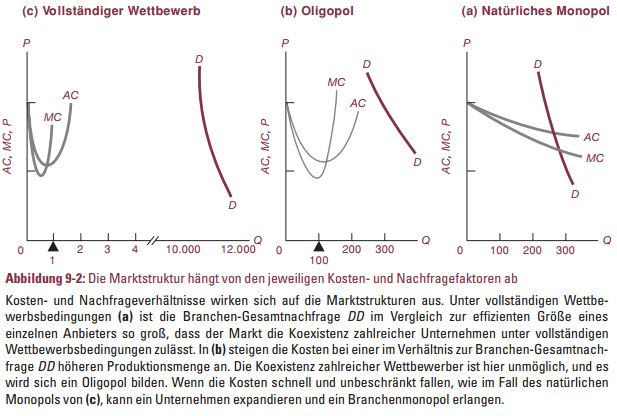
\includegraphics[width=0.98\textwidth]{img/wettbewerb_vergleich.jpg}

\subsubsection{natürliches Monopol}
Ein {\bf natürliches Monopol} ist ein Markt, in dem der Branchenoutput nur von einemeinzigen Unternehmen auf effiziente Weise produziert werden kann. Dieser Fall tritt ein, wenn die Technologie über eine breite Produktionspalette hinweg, die so groß ist wie die gesamte Nachfrage, Skalenvorteile bietet.

\subsubsection{Marktzutrittsbarrieren}
Marktzutrittsbarrieren sind Faktoren, die es neuen Unternehmen schwer machen, in einem Wirtschaftszweig Fuß zu fassen.
\begin{itemize}
\item {\bf Skaleneffekte}
\item {\bf Gesetzliche Beschränkungen.} z.B. Patente, Lizenzen, Importbeschränkungen
\item {\bf Hohe Zutrittskosten } z.B. Planung, Entwicklung und Test eines neuen Flugzeugs
\item {\bf Werbung und Produktdifferenzierung} Die Nachfrage nach jedem der individuell differenzierten Produkte ist so gering, dass es dadurch nur wenigen Unternehmen möglich ist, am tiefsten Punkt ihrer U-förmigen Kostenkurve zu operieren.
\end{itemize} 

\subsection{Grenzerlös und Monopol}
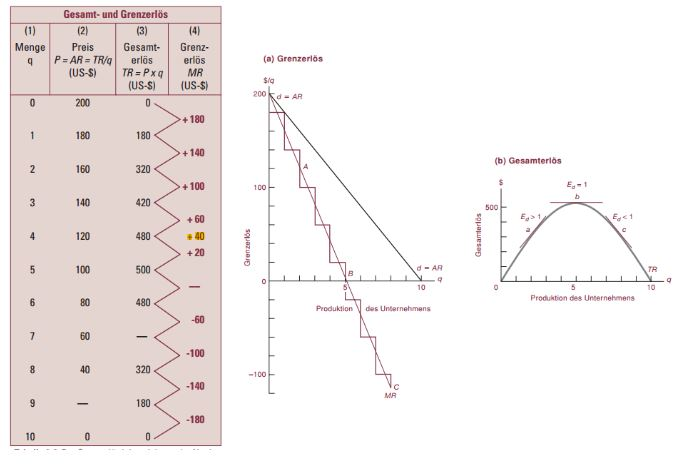
\includegraphics[width=0.98\textwidth]{img/grenzerlos.jpg}

Graphiken:\\
(a) Die rostfarbenen Stufen zeigen die Anstiege des Gesamterlöses aus jeder zusätzlichen Produktionseinheit. MR fällt von Anfang an unter P. MR wird mit unelastischer dd negativ. Eine Glättung der ansteigenden MRStufen ergibt die durchgängige, dünne rostfarbene MR- Kurve, die im Falle der geradlinigen dd immer eine doppelt so hohe Steigung wie dd haben wird.\\
(b) Der Gesamterlös weist eine glockenförmige Kurve auf – Anstieg von null, wobei q = 0, bis zu einem Maximum (wo dd eine Elastizität von 1 aufweist), danach neuerlicher Abfall auf null, wobei P = 0. Die Steigung von TR ergibt die geglätteten MR, ebenso wie der in Sprüngen anwachsende TR die ansteigenden MR-Stufen widerspiegelt.

\subsubsection{Grenzerlös und Preis}
Der Grenzerlös (MR) ist die Erhöhung des Erlöses, die durch eine zusätzlich verkaufte Einheit entsteht. Der MR kann dabei positiv oder negativ sein.\\
Bei abwärtsgerichteter Nachfragekurve gilt:
\begin{equation}
P > MR \text{ ( = P – geringerer Erlös für alle vorherigen q ) } \nonumber
\end{equation}
\subsubsection{Elastizität und Grenzerlös}
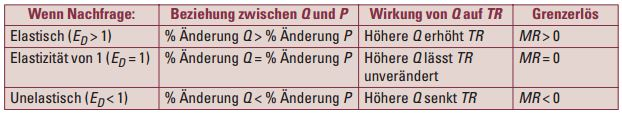
\includegraphics[width=0.88\textwidth]{img/grenzerlos_elas.jpg}
\subsubsection{Gewinnmaximierende Bedingungen}
 Definitionsgemäß entspricht der
Gesamtgewinn dem Gesamtertrag abzüglich
der gesamten Kosten; in Symbolen:
\begin{equation}
TP = TR – TC = (P * q) – TC \nonumber
\end{equation}
Daraus leitet sich die wichtige Erkenntnis ab, dass das Gewinnmaximum dann erreicht wird, wenn die Produktionsmenge so groß ist, dass der Grenzerlös des Unternehmens seinen Grenzkosten entspricht.\\
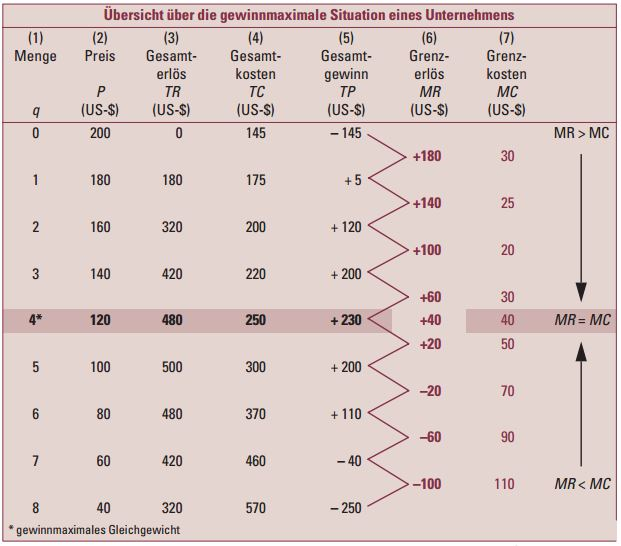
\includegraphics[width=0.98\textwidth]{img/situation.jpg}\\

Das {\bf Gewinnmaximum } eines Monopolisten wird bei jenem Preis (P*) und jener Menge (q*) erreicht, bei denen der Grenzerlös genau den Grenzkosten entspricht:\\ 
MR = MC, bei P* und q* mit dem größtmöglichen Gewinn.\\
\newpage
\begin{wrapfigure}{l}{0.5\textwidth}
  \begin{center}
  	\vspace{-10pt}
    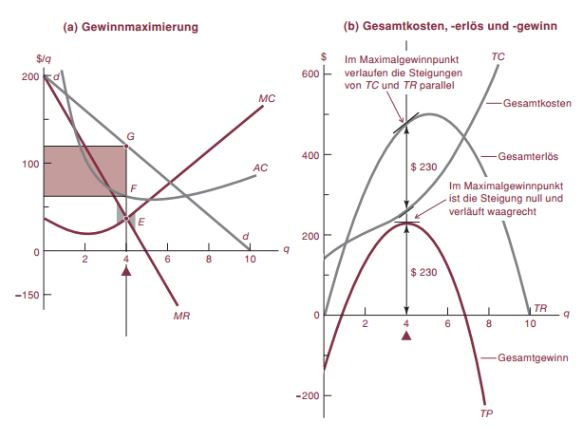
\includegraphics[width=0.48\textwidth]{img/gewinnmaximierung.jpg}
    \vspace{-10pt}
    \end{center}
\end{wrapfigure}
(a) In E, wo die MC- die MR-Kurve schneidet, liegt die Gleichgewichtsposition des Maximalgewinns. Jede Bewegung weg von E geht mit einem Gewinnrückgang einher. Der Preis liegt auf der Nachfragekurve in Punkt G über E; und da P über AC liegt, ist der Maximalgewinn positiv. (Können Sie erklären, warum das rostfarbig unterlegte Rechteck den Gesamtgewinn misst? Und warum die grau unterlegten Dreiecke beiderseits von E den Rückgang des Gesamtgewinns ausweisen, der sich aus einer Abweichung von MR = MC ergäbe?)\\
(b) Dieses Bild enthält die gleiche Aussage bezüglich der Gewinnmaximierung wie (a), verwendet aber die Gesamtkonzepte anstelle der Grenzkonzepte. Die TR-Kurve zeigt den Gesamterlös, während die TC-Kurve die Gesamtkosten darstellt. (Warum nimmt TR bei q = 0 und bei q = 10 den Wert 0 an?) Der Gesamtgewinn (TP) entspricht TR – TC oder geometrisch betrachtet der vertikalen Distanz von TC nach TR. Am Punkt des maximalen Gewinns ist die Differenz zwischen der Gesamterlös- und der Gesamtkostenkurve am größten. Die Steigung jeder Kurve entspricht ihrem Grenzwert (beispielsweise entspricht die Steigung von TR dem MR). Am Gewinnmaximum verlaufen TR und TC parallel und weisen daher eine identische Steigung MR = MC auf.
\subsubsection{Vollständiger Wettbewerb als Grenzfall des unvollständigen Wettbewerbs}
Unter Bedingungen des vollständigen Wettbewerbs entspricht der Preis dem Durchschnittserlös, der seinerseits dem Grenzerlös entspricht (P = MR = AR). Die dd-Kurve und die MR-Kurve eines Unternehmens im vollständigen Wettbewerb fallen als horizontale Linien zusammen. \\
Da ein Unternehmen im vollständigen Wettbewerb jede beliebige Menge zum Marktpreis verkaufen kann, gilt am Punkt des maximalen Gewinns: MR = P = MC

\subsubsection{Marginalprinzip}
Dies ist das Marginalprinzip, das besagt, dass jedermann seine Gewinne oder seine Bedürfnisbefriedigung maximiert, indem er nur Grenzkosten und Grenznutzen einer Entscheidung berücksichtigt. Es gibt unzählige Situationen, in denen sich dieses Marginalprinzip anwenden lässt. Wir haben soeben gesehen, dass das Marginalprinzip des Ausgleichs von Grenzkosten und Grenzerlös die Regel für die Gewinnmaximierung von Unternehmen ist. Ein weiteres Anwendungsbeispiel sind kluge Investitionsentscheidungen. Wenn eine Entscheidung getroffen werden muss, beispielsweise ob man in ein Unternehmen investieren oder ein Haus verkaufen sollte, lohnt es sich immer, frühere Gewinne oder Verluste außer Acht zu lassen und nur aufgrund der Grenzerträge und -kosten zu entscheiden. Das Marginalprinzip ist eine der wichtigsten Lektionen der Volkswirtschaft.











\end{document}
